% !TeX document-id = {57f7666b-e03d-5798-4b62-aabfb1296366}
% !TeX TXS-program:compile = pdflatex -synctex=1 -interaction=nonstopmode -output-directory=build -jobname=p6_aionfpga_thesis_canzani_mueller thesis.tex
% !TeX TXS-program:bibliography = biber --output-directory build p6_aionfpga_thesis_canzani_mueller
% !TeX TXS-program:glossary = makeglossaries -d build p6_aionfpga_thesis_canzani_mueller
% !TeX TXS-program:view = txs:///view-pdf ./build/p6_aionfpga_thesis_canzani_mueller.pdf

\documentclass[final]{fhnwreport}

%% Packages
% Main packages
\usepackage[english]{babel}
\usepackage[T1]{fontenc}
\usepackage[utf8]{inputenc}
\usepackage{lmodern}
\usepackage{textcomp}
\usepackage{graphicx}
\usepackage{float}

% Useful packages
\usepackage[pdftex,dvipsnames,table,tables]{xcolor}
\usepackage{csquotes}
\usepackage{siunitx}
\usepackage{xfrac}
\usepackage{listings}
\usepackage{lstautogobble}
\usepackage[bottom]{footmisc}
\usepackage{footnote}
\usepackage{verbatim}
\usepackage[textsize=footnotesize]{todonotes}
%\usepackage{xurl}
%\usepackage{url}
%\usepackage{soul}

% TikZ packages
%\usepackage{standalone}
%\usepackage{tikz}
%\usepackage{circuitikz}
%\usetikzlibrary{arrows}
%\usetikzlibrary{calc}
%\usetikzlibrary{intersections}

% Math packages
\usepackage{amsmath}
%\usepackage{amssymb}
\usepackage{array}
%\usepackage{amsthm}

% Table packages
\usepackage{tabularx}
%\usepackage{longtable}
\usepackage{multirow}
\usepackage{multicol}
\usepackage{booktabs}

% Figure packages
%\usepackage{subfig}
\usepackage{caption}
\usepackage{subcaption}

% PDF packages
\usepackage{pdfpages}
\usepackage{pdflscape}

% Other packages
%\usepackage{xargs}

%% Settings
% Bibliography
\usepackage[style=ieee,dashed=false,urldate=comp,backend=biber]{biblatex}
\addbibresource{literature/bibliography.bib}

% Glossary
\usepackage[toc]{glossaries}
\makeglossaries

\newglossaryentry{test}
{
    name=Test,
    description={Just a test}
}


% Graphics
\graphicspath{{./graphics/}}

% Listings
% purple {0.776,0.584,0.776} / yellow {0.976,0.682,0.341} / orange {0.976,0.482,0.341}
\definecolor{keywordcolor}{rgb}{0.925,0.376,0.4} % red
\definecolor{commentcolor}{rgb}{0.651,0.675,0.725} % gray
\definecolor{stringcolor}{rgb}{0.6,0.78,0.58} % green
\definecolor{backgroundcolor}{rgb}{0.976, 0.98, 0.98} % light gray

\lstdefinestyle{C++}{
    autogobble,
    backgroundcolor=\color{backgroundcolor},
    commentstyle=\color{commentcolor},
    keywordstyle=\color{keywordcolor},
    numberstyle=\tiny\color{commentcolor},
    stringstyle=\color{stringcolor},
    basicstyle=\ttfamily\footnotesize,
    breakatwhitespace=false,
    breaklines=true,
    breakautoindent=true,
    breakindent=50pt,
    escapeinside={(*}{*)},
    captionpos=b,
    keepspaces=true,
    numbers=left,
    numbersep=5pt,
    showtabs=false,
    showspaces=false,
    showstringspaces=false,
    tabsize=2,
    language=C++
}


% Other
%\geometry{twoside=false}
\setlength{\marginparwidth}{2cm}
\overfullrule=5em

%% Custom definitions
% Table definitions
\newcolumntype{L}[1]{>{\raggedright\arraybackslash}p{#1}}
\newcolumntype{C}[1]{>{\centering\arraybackslash}p{#1}}
\newcolumntype{R}[1]{>{\raggedleft\arraybackslash}p{#1}}
\newcolumntype{M}[1]{>{\centering\arraybackslash}m{#1}}
\newcolumntype{N}{@{}m{0pt}@{}}

% Month
\newcommand{\MONTH}{
	\ifcase\the\month
	\or January
	\or February
	\or March
	\or April
	\or May
	\or June
	\or July
	\or August
	\or September
	\or October
	\or November
	\or December
	\fi}

% URL
\urlstyle{same}

% siunitx
\sisetup{per=fraction}



\title{\textbf{{\Huge AI High-Performance Solution \\[2mm] on FPGA}}}
\author{\textit{{\LARGE Bachelor Thesis}}}
\date{}

\begin{document}

% Title page
\selectlanguage{english}
\pagenumbering{gobble}
\maketitle

\begin{figure}[H]
  \centering
  \includegraphics[width=0.55\textwidth]{top_assembly}
\end{figure}

\vfill
\begin{center}
  \begin{tabular}{>{\bfseries\large}rl}
    Degree Program & Electrical Engineering and Information Technology \\[2mm]
    Customer       & Institute for Sensors and Electronics \\[2mm]
    Coaches        & Prof. Michael Pichler, Prof. Dr. Hanspeter Schmid \\[2mm]
    Expert         & Dr. J\"urg M. Stettbacher \\[2mm]
    Team           & Nico Canzani, Dominik M\"uller \\[2mm]
    Date           & \today
  \end{tabular}
\end{center}
\clearpage

% Abstract
\pagenumbering{roman}
\chapter*{Abstract}
\todo[inline]{needs to be updated}
% Motivation
In a world of self-driving cars and automated quality control in manufacturing, real-time image classification is becoming increasingly important.
Artificial intelligence, and deep learning in particular, are achieving excellent classification accuracies, but there are some challenges.
% Problem statement
For one thing, high-resolution image acquisition systems require a lot of processing power.
For another, a large labeled dataset of training data is required to train deep convolutional neural networks.
% Approach
A solution for the former is to use field-programmable gate arrays as hardware accelerators.
The focus of this project, however, is to collect a labeled dataset.
For this purpose, an industrial camera with a frame rate of \SI{200}{fps} is used to acquire images of 22 different throwing objects.
To simplify this task, a camera throw detection mechanism is implemented and various Python scripts are used.
% Results
The developed software uses an image change detection algorithm to detect individual throws.
The result is a fully labeled dataset that consists of more than \num{15000} usable images with at least 480 images of each object.
% Conclusions
Developing software to support the image acquisition proved to be extremely useful.
It made it possible to collect the complete dataset in only two days.

% from https://users.ece.cmu.edu/~koopman/essays/abstract.html

\vspace{1cm}
\begin{tabular}{>{\bfseries}ll}
  Team  & Nico Canzani, Dominik M\"uller \\
  Keywords & Artificial Intelligence, FPGA, Convolutional Neural Network % Industrial Camera
\end{tabular}

\clearpage

% Declaration of Authenticity
\chapter*{Declaration of Authenticity}

We, the undersigned, declare that all material presented in this paper is our own work or fully and specifically acknowledged wherever adapted from other sources.
We understand that if at any time it is shown that we have significantly misrepresented material presented here, any degree or credits awarded to us on the basis of that material may be revoked.

We declare that all statements and information contained herein are true, correct and accurate to the best of our knowledge and belief.
% This paper or part of it has not been submitted for any other academic award.

\vspace{1cm}
\begin{table}[h]
  \renewcommand{\arraystretch}{1.5}
  \begin{tabularx}{\textwidth}{C{5cm} >{\centering}X C{5cm}}
     & & \\ \cline{1-1} \cline{3-3}
    Nico Canzani & \today & Dominik M\"uller \\
  \end{tabularx}
\end{table}

\clearpage

% Contents
\tableofcontents
\clearpage

% Chapters
\pagenumbering{arabic}
\chapter*{Introduction}
\addcontentsline{toc}{chapter}{Introduction}
\markboth{Introduction}{}
\label{ch:introduction}

Humanity has been trying to understand how thinking works for thousands of years and is making considerable progress.
One of the newest fields in science and engineering is \acrfull{ai}, which goes even further than just understanding the thinking process.
It attempts to build intelligent entities \cite{ai}.
For example, in most vehicles today, the human being chooses which reaction is the best.
However, humans are influenced, distracted and have reaction times that are simply too slow to avoid accidents.
When these tasks are delegated to a computer, a background task is required that is capable of identifying threats and reacting appropriately.
For this purpose, images must be acquired and evaluated.
Since the dangers are not always the same, intelligence is required to make the decisions.
This is where \acrshort{ai} comes into play.
The progress in the field of self-driving cars through \acrshort{ai} has been considerable in the recent years.
All Tesla vehicles now in production are equipped with full self-driving hardware and require only a software update to replace the driver \cite{tesla_self_driving_cars}.
Another example is optical quality control.
Thanks to computers, the accuracy can be optimized and the throughput can be increased compared to human labor.
Both examples require fast and accurate image recognition, which is usually performed by a so-called \acrfull{cnn}.

In order to keep up with the current state of development, the institute for sensors and electronics (ISE) which is part of the University of Applied Sciences and Arts Northwestern Switzerland (FHNW) has launched this project, which deals with these two aspects.

This project has two main objectives:

\begin{enumerate}
	\item Showing the FHNW how to run hardware accelerated \acrshort{ai}
	\item Developing an eye-catcher for the ISE, which can be presented at trade fairs
\end{enumerate}

Apart from the hardware, which is an Ultra96-V2 development board, the procedure was not defined more precisely, which allowed a certain leeway.
The task was defined more precisely by the students as follows:

To meet the requirements of fast image recognition, objects are thrown past a high-speed camera.
These objects are taken from a set of 22 items such as a floorball or a stuffed bunny.
The \acrshort{cnn} shall be described and trained with an end-to-end open-source platform for machine learning called Tensorflow \cite{tensorflow_main}.
The throwing booth should function as a plug-and-play device.
This makes it easier to use at a trade fair.
Appendix \ref{app:problem_statement} shows the task definition.

During the previous project, the throwing booth was designed and built.
An industrial camera and suitable lighting were evaluated, purchased and installed.
Furthermore, a dataset was collected, which consists of more than \num{15000} usable frames with at least \num{485} frames of each object.
Each frame in the dataset is labeled and therefore indicates what kind of object it is.
% For each image in the database, labels have been set to indicate what kind of object it is.
% Also it is noted if the picture is not good (for example because a hand was on the picture) or if the object is cut off at the edge of the image.

In this project an \acrfull{os} for the processor of the Ultra96-V2 is set up.
The \acrshort{os} can control the \acrfull{fpga}, which is included in the \acrfull{mpsoc}.
On this \acrshort{fpga} a \acrfull{dpu} is implemented, which performs the high-speed image recognition.
% The trained neural network was quantized before.
% This makes it possible to execute the image recognition by using C-code commands. % why C-code?
The results are verified for accuracy and throughput.

This thesis contains seven main parts.
The first part is the theoretical background about \acrfull{ai}.
The second part describes the training of the \acrlong{cnn}.
Next comes a chapter that describes the throwing booth.
The chapter embedded platform introduces two operating systems and describes how to use them.
The inference application is described in the chapter inference.
The results of the \acrshort{cnn} are documented in the chapter verification.
After these chapters there is a conclusion and our personal experiences with Xilinx, Avnet and TensorFlow.

All components developed for this project fall under the Apache 2.0 license and are freely available on GitHub (\url{https://git.io/aionfpga}).

\chapter{Theoretical Background}
\label{ch:theoretical_background}

This chapter briefly provides the required theory to understand the design process of \acrfullpl{cnn}.
It introduces \acrfull{ai}, \acrfull{ml} and \acrfullpl{ann} in general and focuses on \acrshortpl{cnn}.

\section{Artificial Intelligence}
\label{sec:theoretical_background:ai}

The field of \acrlong{ai} is a branch of computer science that aims to understand and build intelligent entities \cite[p.~1--18]{ai}. % p.~18 / p.~1

\section{Machine Learning}
\label{sec:theoretical_background:ml}

\Acrlong{ml} is a branch of \acrlong{ai} that essentially aims to give computers the ability to learn from data.
Therefore, it deals with the study of algorithms that computers use to perform certain tasks without using explicit instructions \cite[p.~97]{deeplearningbook}.

% ------------------------
\paragraph{Generalization}
The goal of the learning process is to generalize and not to memorize the samples of the training dataset.
A model that fails to generalize can be subject to underfitting or overfitting.
On the one hand, underfitting occurs when the model is not able to reach an acceptable classification accuracy.
Overfitting, on the other hand, refers to the situation where the gap between the training accuracy and the validation accuracy is too large \cite[p.~108--114]{deeplearningbook}.

% ----------------------------------------------
\paragraph{Supervised and Unsupervised Learning}
\Acrlong{ml} algorithms can generally be divided into supervised and unsupervised learning algorithms.
The distinction is based on the type of datasets used during training \cite[p.~102--105]{deeplearningbook}.

Supervised learning algorithms use labeled datasets to learn.
The algorithm takes a guess on a piece of data from the dataset and this guess is then checked against the label (i.e. the correct answer).
This enables the algorithm to adjust itself and therefore to improve future predictions.

Unsupervised learning algorithms, however, work with unlabeled data and therefore only operate on the input data.
The algorithm must learn to make sense of the input data, as it has no means of correcting itself.
Unsupervised learning is usually used in problems that involve finding groups in data or summarizing the distribution of data.

% -----------------------
\paragraph{Deep Learning}
Deep learning is a subset of \acrlong{ml} that was developed to achieve better results than traditional algorithms.
Deep learning algorithms are combinations of a dataset, a cost function, an optimizer and a model.
The best results are achieved by using deep learning architectures in combination with large datasets.
The word \textit{deep} in \textit{deep learning} refers to the large number of layers in a network \cite[p.~151--152]{deeplearningbook}.

\section{Artificial Neural Network}
\label{sec:theoretical_background:ann}

% An \acrlong{ann} is a model used in \acrshort{ml}, % p.~727--
An \acrlong{ann} is a model used in \acrshort{ml} which consists of artificial neurons and weighted connections between those neurons.
% It usually consists of an input layer, several hidden layers and an output layer.
They usually features an input layer, several hidden layers and an output layer.
The individual layers consist of an arbitrary number of artificial neurons, which are connected to one another \cite[p.~33-36]{nn}.

% The simplest \acrshort{ann} is the feedforward neural network, where the information flows in only one direction.
The simplest \acrshort{ann} is the feedforward neural network, where the information propagates in only one direction.
% artificial neurons
% sums up inputs + bias
% applies activation function
% A common propagation function is the weighted sum of the neurons from the previous layer.
A common propagation function is the weighted sum of the neurons from the previous layer.
% The output of each neuron is multiplied with the weight ascociated to the connection between the two neurons.
Therefore, the output of each neuron $i$ is multiplied with the weight $w_{i, j}$ ascociated to the connection between the two neurons.
% These values are then summed up and a bias term is added.
% These values are then summed up and added to a bias term.
These values are summed up and added to a bias term.
In a last step, an activation function is applied, which results in equation \ref{eq:artificial_neuron}.

\begin{equation}
  % y_j = a\left(\sum\limits_{i=1}^{m} (x_i \cdot w_{i, j}) + b\right)
  % y_j = a\left(\sum\limits_{i=1}^{m} x_i w_{i, j} + b\right)
  y_j = a\left(\sum\limits_{i} x_i \cdot w_{i, j} + b\right)
  \label{eq:artificial_neuron}
\end{equation}

where

\begin{tabular}{lll}
  $y_j$ & = & output of neuron $j$ \\
  $a(.)$ & = & activation function \\
  % $m$ & = & number of neurons in the previous layer \\
  $x_i$ & = & output of neuron $i$ from the previous layer \\
  $w_{i, j}$ & = & weight $i, j$ connecting the output of neuron $i$ with the input of neuron $j$ \\
  $b$ & = & bias \\
\end{tabular}
\\




\subsection{Activation Function}
\label{subsec:theoretical_background:ann:activation_function}

An activation function is responsible for transforming the input of an artificial neuron to its output.
% Activation functions are used to introduce a nonlinearity.
% They are usually used to introduce a nonlinearity to to solve problems which are not trivial.
There exists a variety of different linear and non-linear activation functions.
However, non-linear activation functions are preffered due to their ability to learn more complex structures in the data.
The sigmoid and hyperbolic tangent activation functions were traditionally very popular but they both suffer from a saturation problem.
% Most commonly, the \acrfull{relu} activation function is used, which is shown in equation \ref{eq:relu}.
% At the moment, the \acrfull{relu} activation function is  the most commonly used activation function is the \acrfull{relu} activation function
% The \acrfull{relu} activation function is currently the most commonly used.
Currently, the \acrfull{relu} is the most commonly used activation function in the field of deep learning.
It is a piecewise-defined function, which outputs the input if it positive and zero otherwise.
This is shown in equation \ref{eq:relu}.
Furthermore, the \acrshort{relu} activation function requires only a single comparison and is therefore not very computationally expensive \cite{relu}.

\begin{equation}
  a(x) = x^+ = \max(0, x)
  \label{eq:relu}
\end{equation}

% relu (incl. plot)
% maybe sigmoid or tanh

\section{Convolutional Neural Network}
\label{sec:cnn}




\chapter{Training of the CNN}
\label{ch:training_of_the_cnn}

Building a \acrlong{cnn} from scratch leaves a lot of design choices and requires multiple steps.
The first step involves the design of the desired \acrshort{cnn} architecture.
In a second step, the labeled dataset is used to fit the \acrshort{cnn} model.
If necessary, the hyperparameters of the \acrshort{cnn} architecture can be tuned in a third step.

This chapter describes the dataset generation, the design of the \acrshort{cnn} architecture and the actual training of the \acrshort{cnn} model.

\section{Dataset}
\label{sec:training_of_the_cnn:dataset}

The dataset contains frames of 22 different throwing objects, as shown in table \ref{tab:objects}.
It is fully labeled and consists of more than \num{15000} usable frames with at least \num{485} frames of each object.
All frames were collected over the course of two days during the previous project.
Figure \ref{fig:dataset} shows two example frames from the dataset (the \textit{Stuffed Bunny} and the \textit{Hand Featherball}).

\begin{table}
  \caption{List of the different throwing objects}
  \label{tab:objects}
  \centering
  \begin{tabular}{llll}
    \toprule
    \textbf{Objects} &  &  &  \\
    \midrule
    Nerf Dart & American Football & Table Tennis Ball & Shuttlecock \\ % left to right, top to bottom
    Sporf & Arrow & Hand Featherball & Floorball \\
    Spiky Ball & Tesafilm & Sponge & Red Duplo Brick \\
    Green Duplo Brick & Duplo Figure & Foam Die & Infant Shoe \\
    Stuffed Bunny & Goalkeeper Glove & Hemp Cord & Paper Ball \\
    Beer Cap & Water Bottle &  &  \\
    \bottomrule
  \end{tabular}
\end{table}

\begin{figure}[t]
  \centering
  \begin{subfigure}[b]{0.45\textwidth}
    \centering
    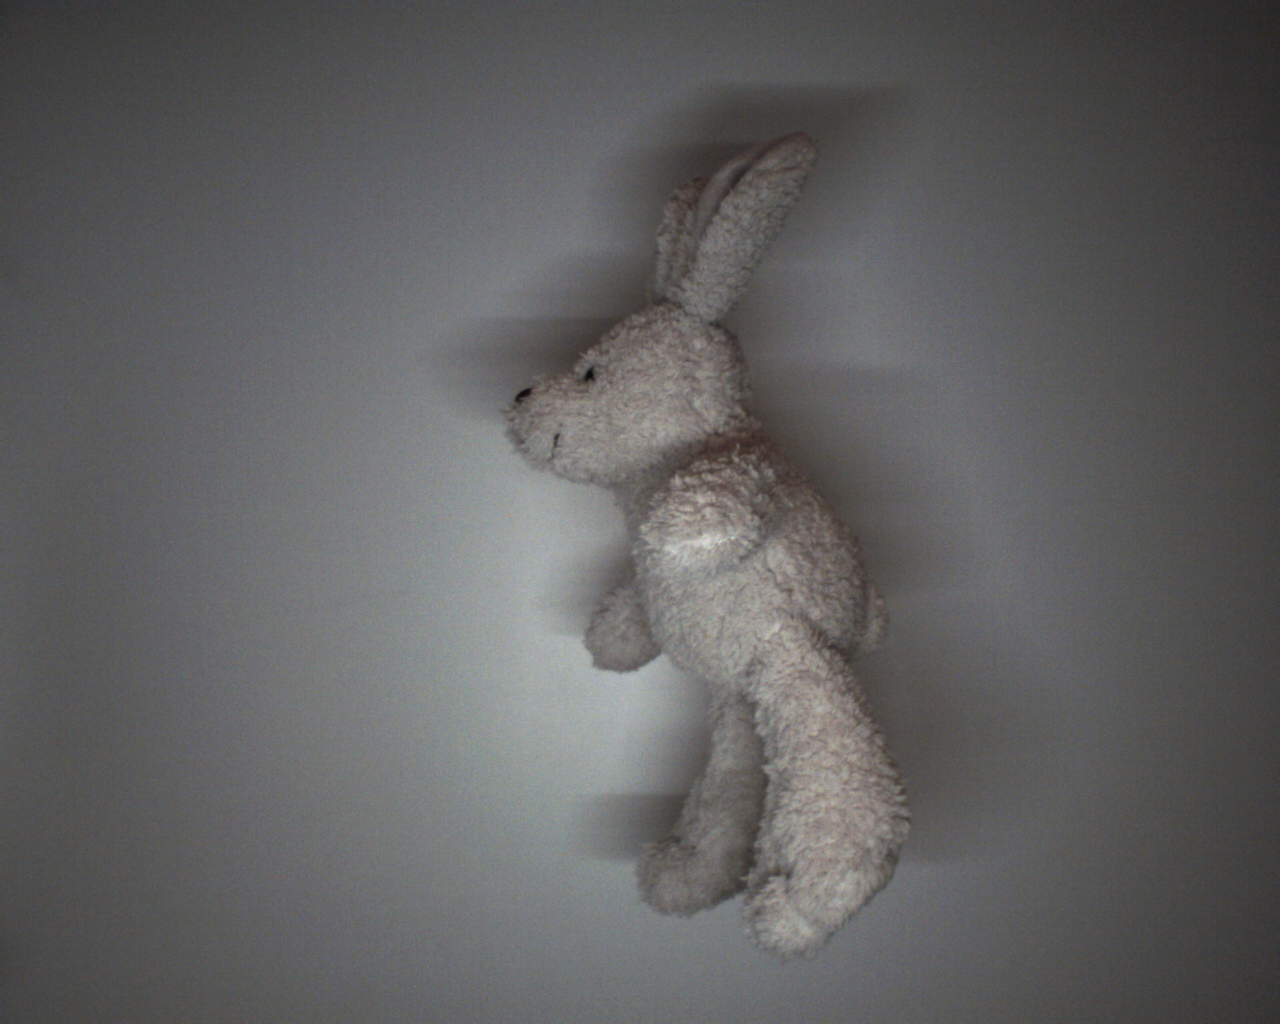
\includegraphics[width=\textwidth]{1574952009_278_10_stuffed-bunny}
    \caption{Stuffed Bunny}
    \label{subfig:dataset_stuffed_bunny}
  \end{subfigure}
  \begin{subfigure}[b]{0.45\textwidth}
    \centering
    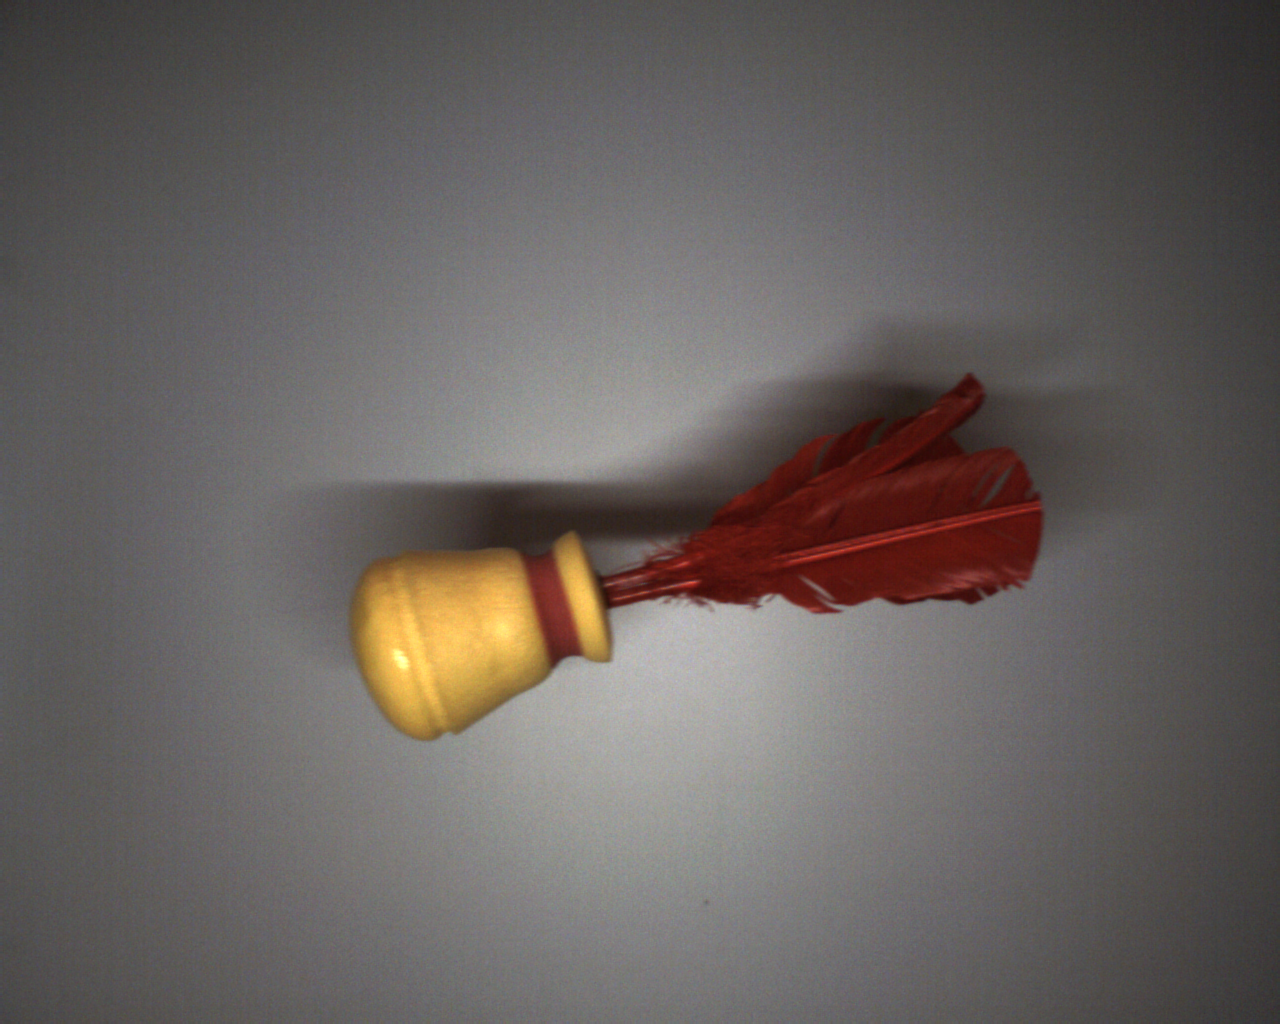
\includegraphics[width=\textwidth]{1574943825_125_8_hand-featherball}
    \caption{Hand Featherball}
    \label{subfig:dataset_hand_featherball}
  \end{subfigure}
  \caption{Two example frames from the dataset}
  \label{fig:dataset}
\end{figure}

% ------------------------------------------------------------------------------------------------------------------------------
\subsection{White Balance}
\label{subsec:training_of_the_cnn:dataset:white_balance}

A notable thing is that on the first day of the data collection, the white balance was performed continuously (every three frames).
This caused the background color of large colored objects to be distorted, as shown in figure \ref{fig:white_balance}.
However, this is not problematic, as noise can improve the generalization and thus reduce overfitting \cite{training_noise}.

\begin{figure}[t]
  \centering
  \begin{subfigure}[b]{0.45\textwidth}
    \centering
    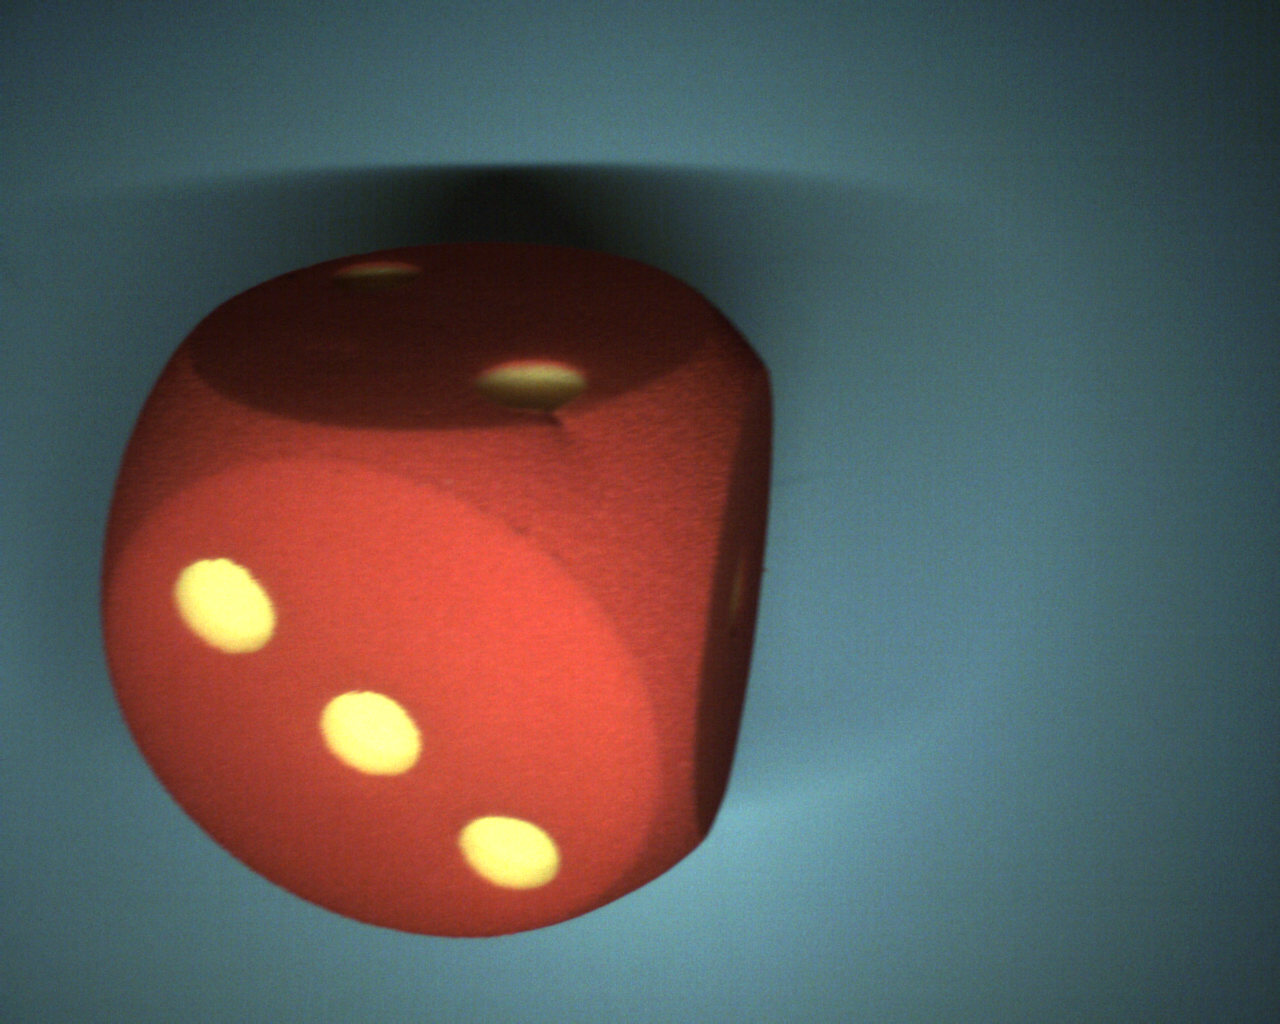
\includegraphics[width=\textwidth]{1574950250_238_9_foam-dice}
    \caption{Continuous white balance}
    \label{subfig:white_balance_first_day}
  \end{subfigure}
  \begin{subfigure}[b]{0.45\textwidth}
    \centering
    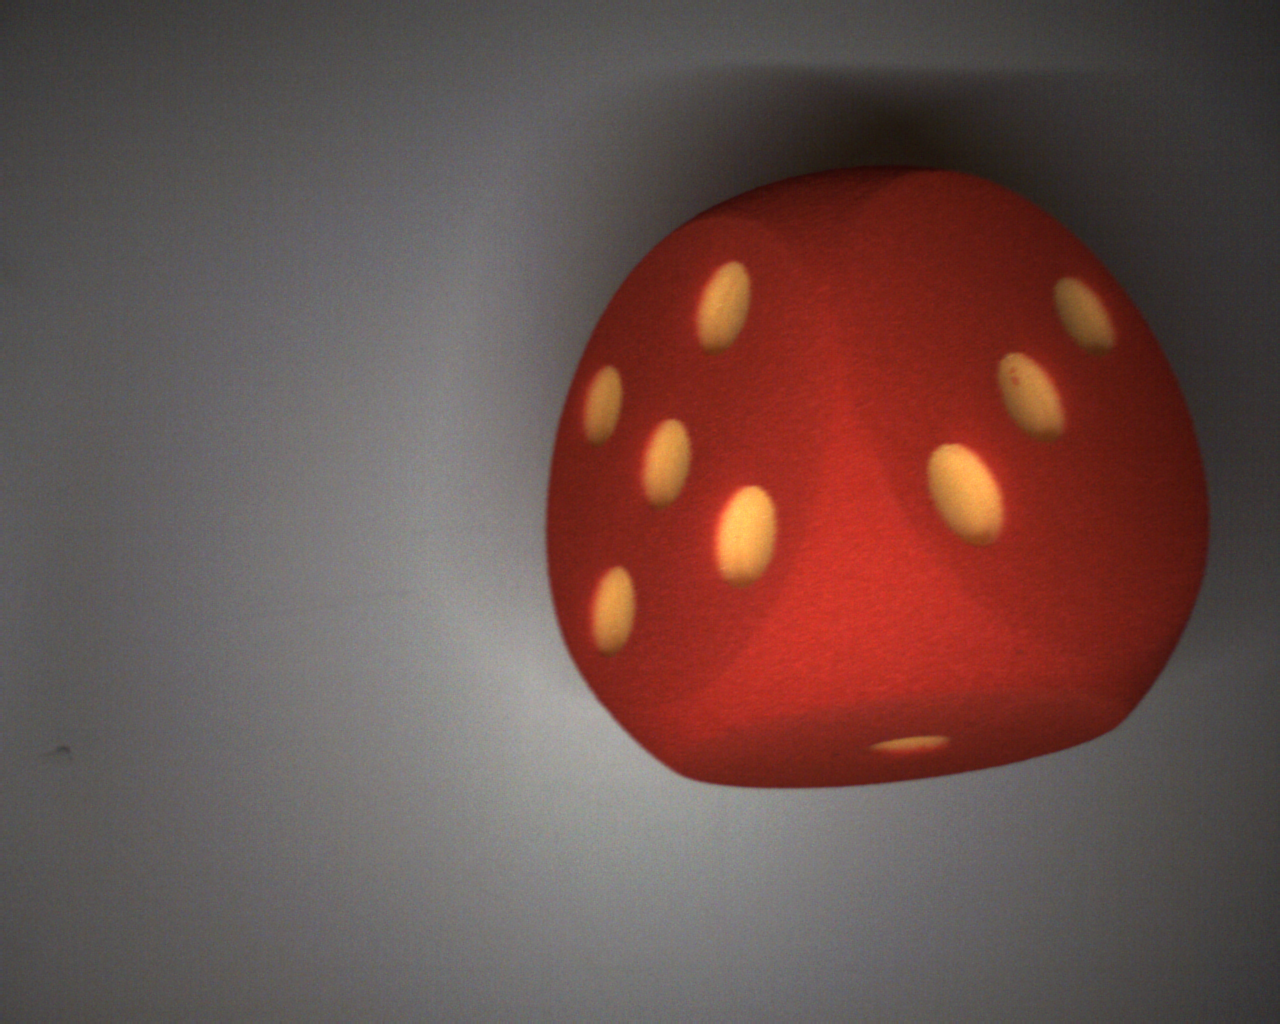
\includegraphics[width=\textwidth]{1575032343_726_8_foam-dice}
    \caption{One-off white balance}
    \label{subfig:white_balance_second_day}
  \end{subfigure}
  \caption{White balance difference between the first (\subref{subfig:white_balance_first_day}) and the second (\subref{subfig:white_balance_second_day}) day}
  \label{fig:white_balance}
\end{figure}

% ------------------------------------------------------------------------------------------------------------------------------
\subsection{Statistics}
\label{subsec:training_of_the_cnn:dataset:statistics}

Figure \ref{fig:statistics} shows the amount of captured frames for each object individually.
It is evident that there are generally more frames of larger objects.
This is, on the one hand, due to the specific implementation of the throw detection mechanism.
On the other hand, the field of view of the camera is not uniformly illuminated (the center is brighter than the edges).
For those reasons, a larger object area is required at the borders to achieve a sufficiently large change in the frame.
However, this also leads to the fact that larger objects are more often only partially in the frame.

The statistics of the dataset reveal that it is slightly imbalanced.
This fact has to be taken into account when creating the various dataset splits (see section \ref{subsec:training_of_the_cnn:dataset:splitting}) that are required for the fitting and evaluation of the model.

An imbalanced dataset can lead to serious problems, e.g. a bias towards the classes with the most samples.
Consider a dataset consisting of only two classes that is imbalanced in such a way that \SI{90}{\percent} of all samples belong to class \texttt{A}.
The fitting process of the classification model will naturally favor class \texttt{A}, since the chance of being right is nine times higher.
The classification could even be independent of the input and always opt for class \texttt{A} (completely ignoring class \texttt{B}).
This obviously terrible classification process would still result in an overall accuracy of \SI{90}{\percent} \cite{training_imbalanced}.

\begin{figure}
  \centering
  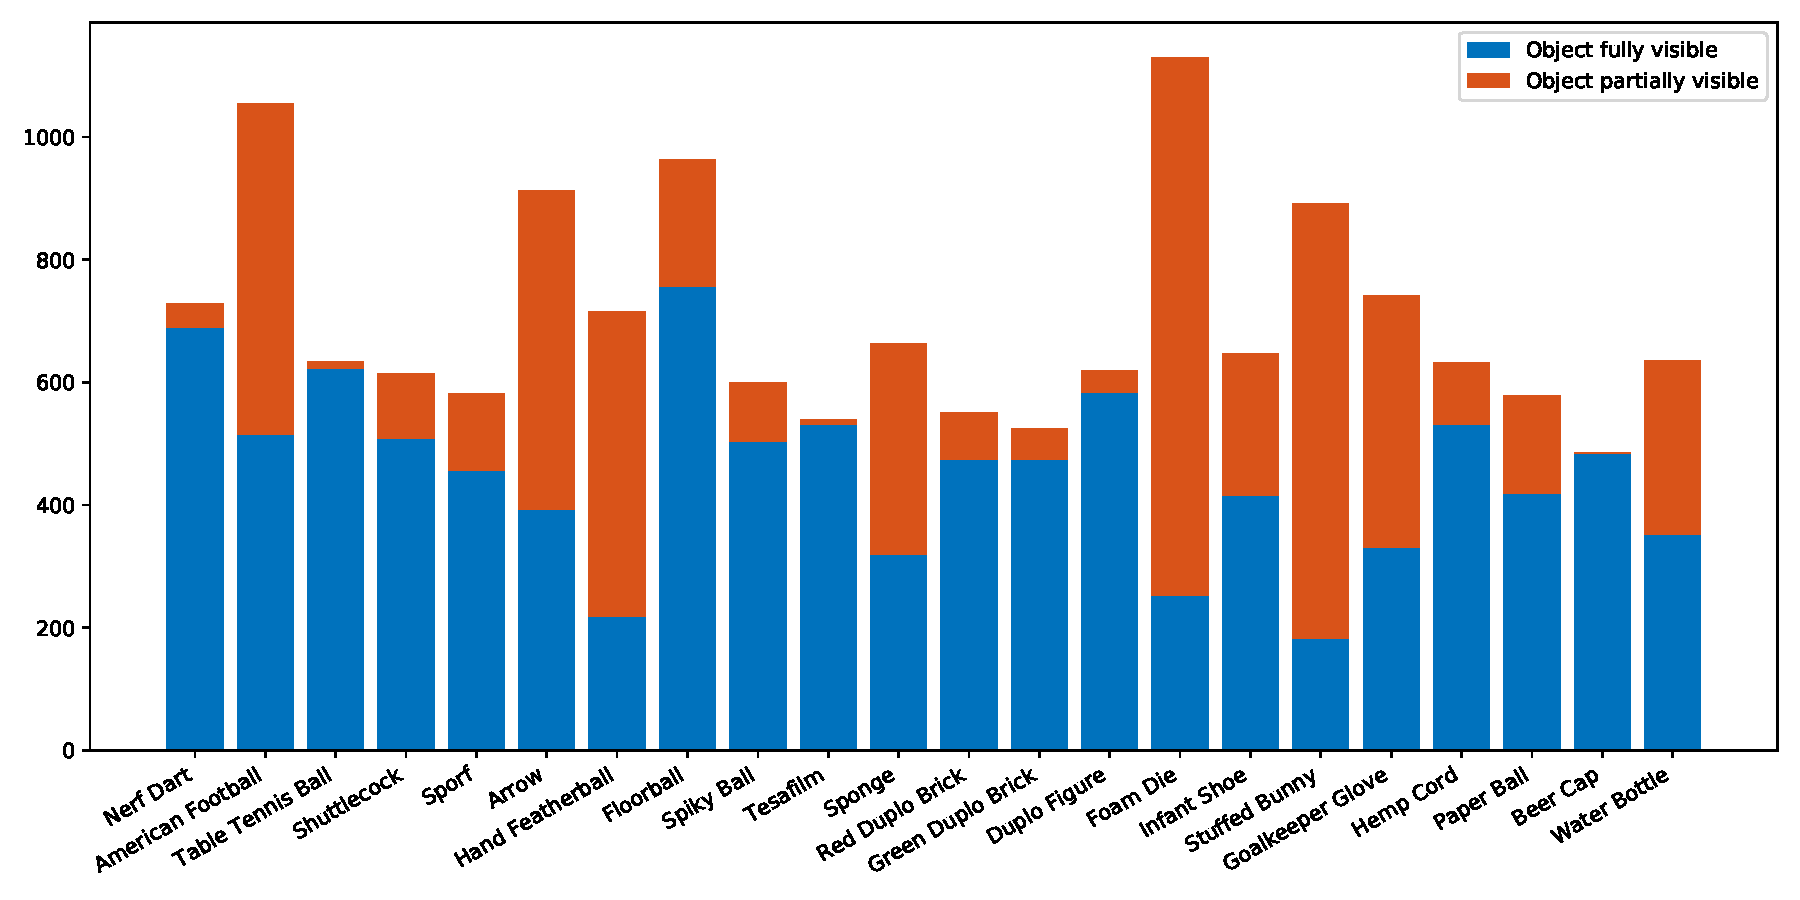
\includegraphics[width=\textwidth]{statistics}
  \caption{Statistics showing the amount of captured frames for each object individually}
  \label{fig:statistics}
\end{figure}

% ------------------------------------------------------------------------------------------------------------------------------
\subsection{Augmentation}
\label{subsec:training_of_the_cnn:dataset:augmentation}

The image dimensions of the individual frames are $1280\times\SI{1024}{px}$ (width $\times$ height) with three color channels (\acrshort{rgb}).
This is an enormous amount of input data for a \acrlong{cnn} and would result in an extremely large amount of mathematical operations to classify even a single frame.
As a result, the classification throughput is reduced and thus the time required to fit the \acrshort{cnn} model is greatly increased.

Another important aspect of the dataset is the fact that it was collected over the course of only two days.
Some objects (e.g. the \textit{Water Bottle}) were even added only on the second day of the data collection.
Real-world observations have shown that the surrounding ambient light and the orientation of an object have a significant influence on the classification performance.
The data collection took place in a relatively dim location and the ambient light did not change much.
The classification performance is therefore much better when there is less ambient light.

Furthermore, the orientation of an object on a frame also impacts the classification performance.
One such problem arises if, for example, the \textit{Shuttlecock} is deliberately thrown with the plastic tail feathers in front of the cork head.
Experiments have shown that this results in a complete misclassification of the object.

For those reasons, a range of image data augmentation techniques are used on the individual frames to improve the real-world classification performance \cite{training_data_augmentation}.
The dataset augmentation is done with the Python script \texttt{dataset\_generator.py}, which uses NumPy as well as the Python implementation of the \acrfull{opencv}.
NumPy provides support for large, multi-dimensional arrays and an assortment of functions to work on these arrays \cite{training_numpy}.
\acrshort{opencv} provides various image transformation functions (e.g. resizing, color space conversions) and conveniently uses NumPy arrays to represent the images \cite{training_opencv_intro}.

% -----------------------
\paragraph{Image Scaling}
To reduce the input data of the \acrshort{cnn} model, the width and height of the individual frames are each scaled down by a factor of four.
This results in an image with the dimensions of $320\times\SI{256}{px}$ (width $\times$ height) and thus in a data reduction of \num{16}.

These dimensions are great because even the important features of the smallest objects are still preserved.
Given that the background of the frames remains more or less the same, a reasonably deep \acrshort{cnn} should have no problems distinguishing between the only \num{22} different classes.

The downsampling is achieved with the use of nearest-neighbor interpolation.
This results in more noise and scaling artifacts than other interpolation methods, such as bilinear or bicubic interpolation.
The scaling artifacts shown in figure \ref{fig:augmentation_downsampling} are the result of aliasing.
The advantages of nearest-neighbor interpolation are its simplicity and fast execution time \cite{training_interpolation}.
Furthermore, the additional noise can improve the generalization and therefore reduce overfitting \cite{training_noise}.

The Python implementation of the image scaling makes use of the \acrshort{opencv} function \texttt{cv2.resize}.
This function is supplied with three arguments: the NumPy array that represents the image, the desired output image size and the interpolation method \cite{training_opencv_resize}.

\begin{figure}
  \centering
  \begin{subfigure}[b]{0.45\textwidth}
    \centering
    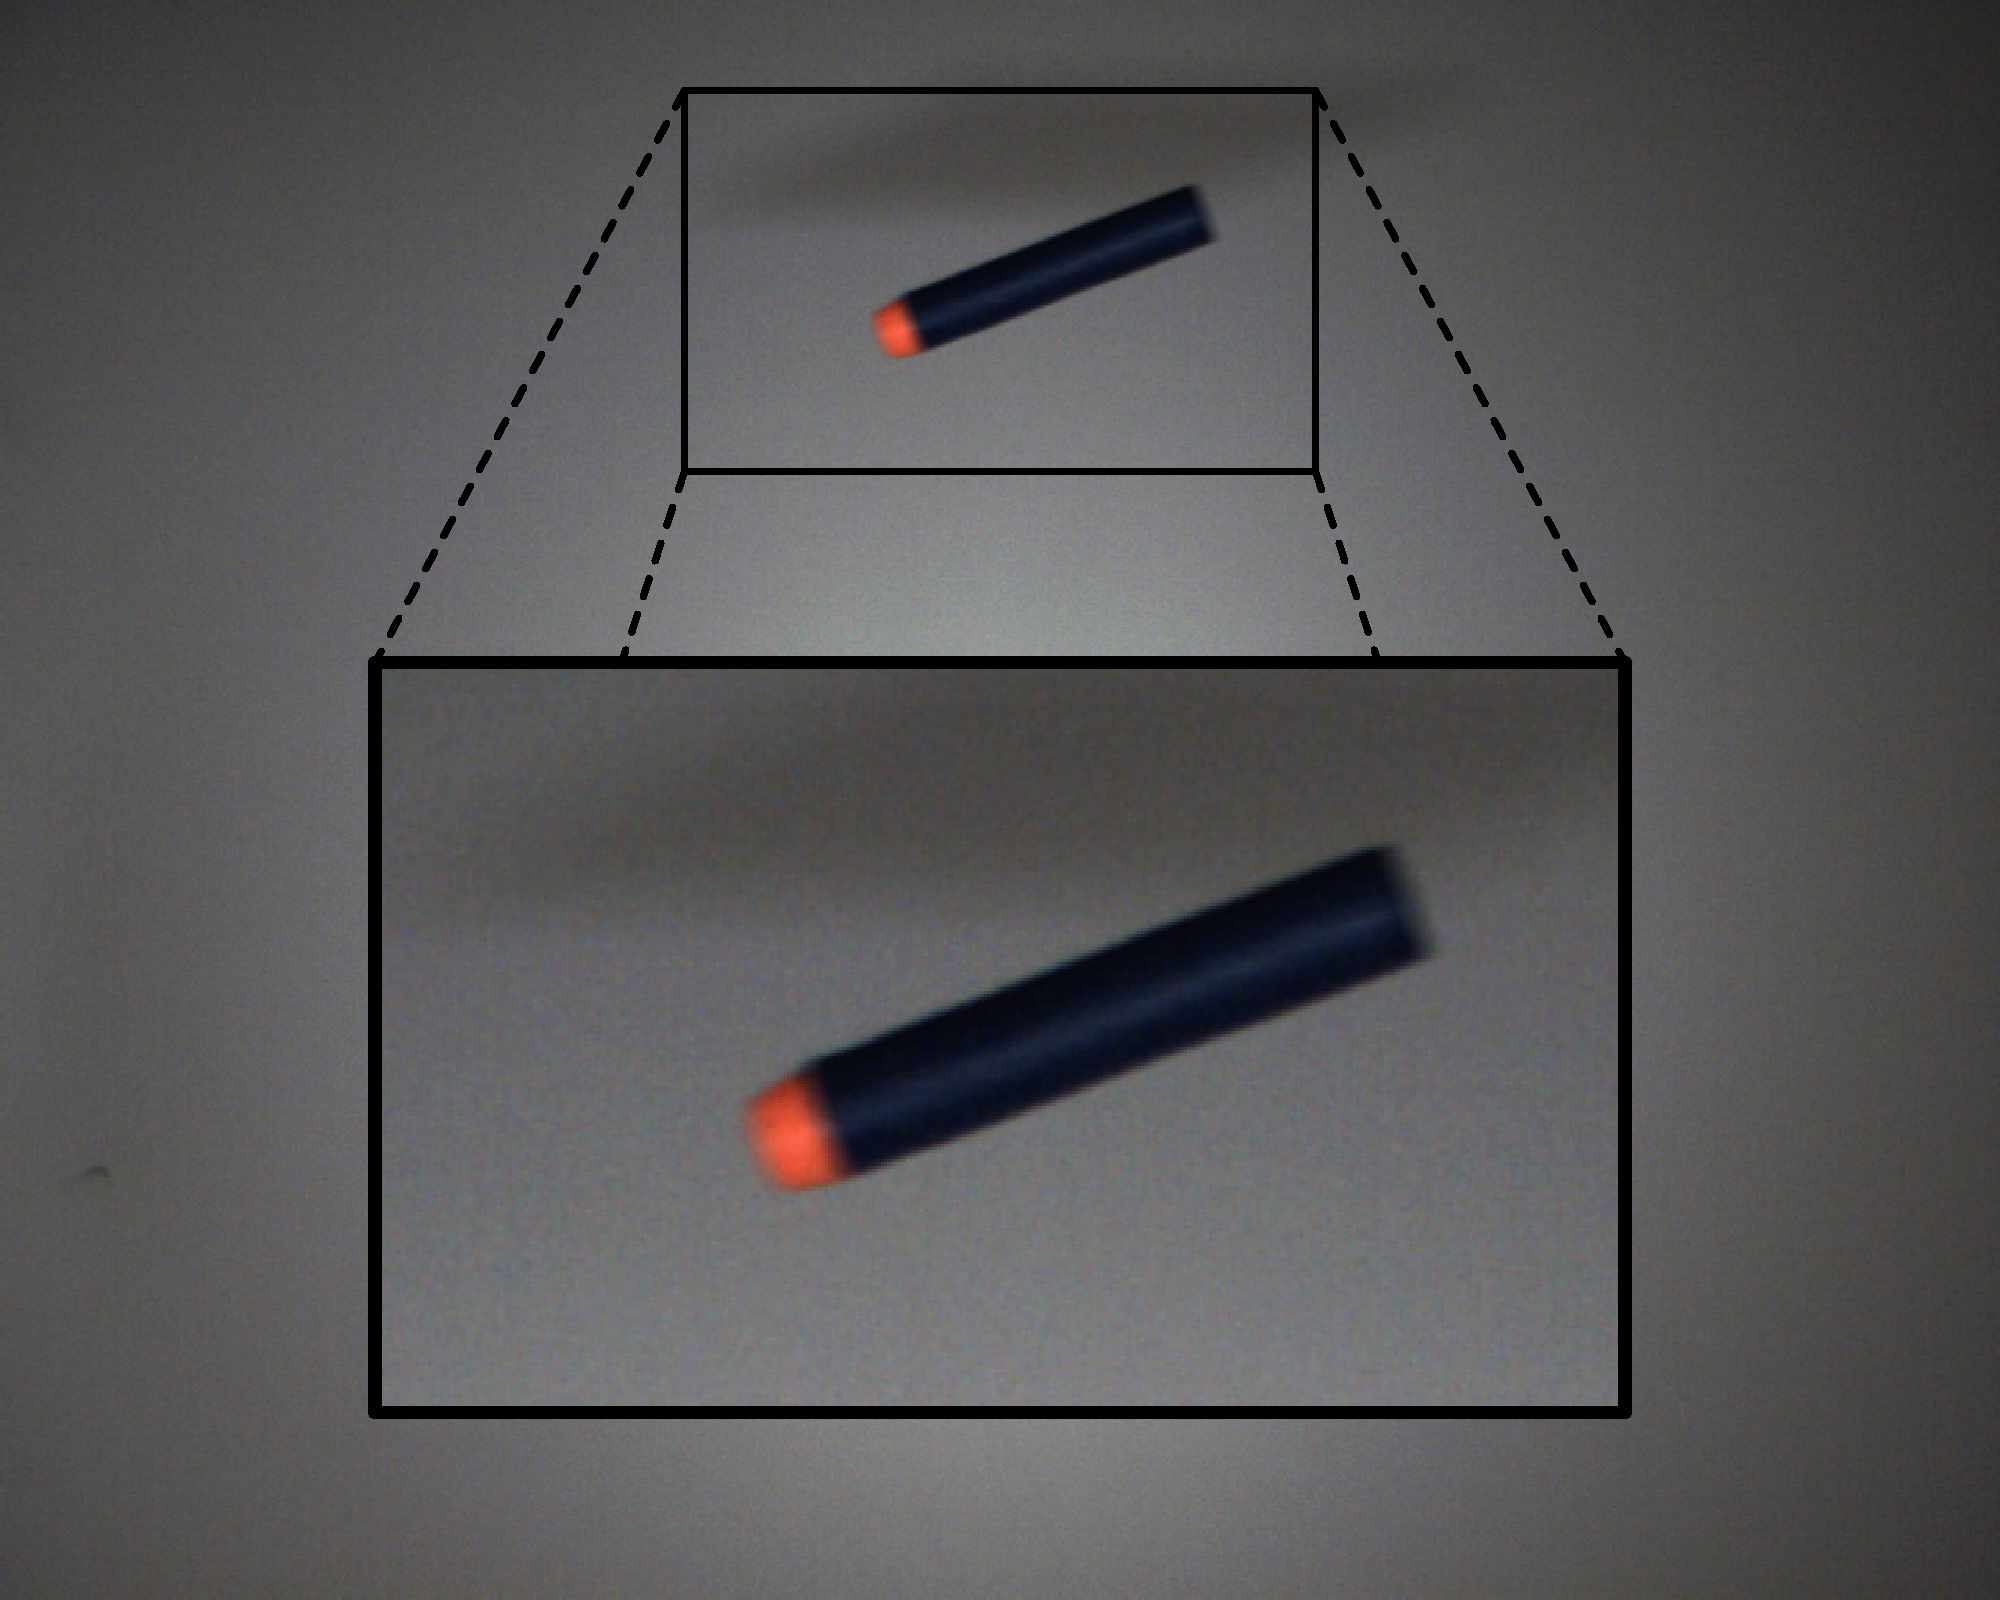
\includegraphics[width=\textwidth]{augmentation_downsampling/1575032863_742_3_nerf-dart_zoom}
    \caption{Original version}
    \label{subfig:ad_original}
  \end{subfigure}
  \begin{subfigure}[b]{0.45\textwidth}
    \centering
    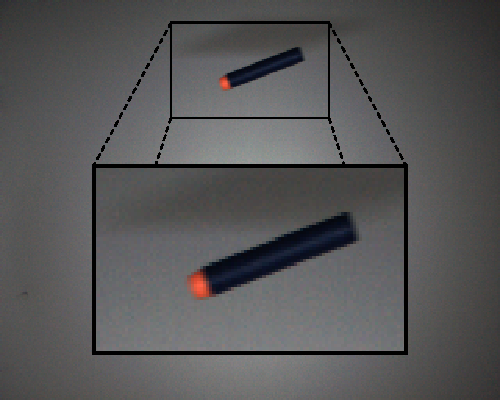
\includegraphics[width=\textwidth]{augmentation_downsampling/1575032863_742_3_nerf-dart_resized_zoom}
    \caption{Scaled-down version}
    \label{subfig:ad_resized}
  \end{subfigure}
  \caption{Example of an original (\subref{subfig:ad_original}) and a scaled-down version (\subref{subfig:ad_resized}) of a frame ($2\times$ inner zoom added to better highlight the difference)}
  \label{fig:augmentation_downsampling}
\end{figure}

% ---------------------
\paragraph{Color Space}
To reduce the dependence on ambient light intensity, the average brightness of the individual frames is changed.
The rounded average brightness $B$ of an image can be calculated using equation \ref{eq:rounded_average_brightness}.
This equation is implemented in Python with the help of the NumPy function \texttt{np.sum}, which computes the sum of all array elements \cite{training_numpy_sum}.

\begin{equation}
  B = \left\lfloor\frac{1}{w\cdot h\cdot c} \cdot \sum\limits_{k=1}^c \sum\limits_{i=1}^h \sum\limits_{j=1}^w \boldsymbol{M}_{ij}^{k} + 0.5\right\rfloor
  \label{eq:rounded_average_brightness}
\end{equation}

where

\begin{tabular}{lll}
  $B$ & = & rounded average brightness \\
  $w$ & = & width of the image \\
  $h$ & = & height of the image \\
  $c$ & = & number of channels \\
  $\boldsymbol{M}^k$ & = & pixel matrix of channel $k$ \\
\end{tabular}
\\

\clearpage

The rounded average brightness of the background was computed at various times of the day and lies between \numrange{85}{160}.
This range includes environments without ambient light as well as environments with indirect sunlight and artificial ambient light.
In the light of these results, a step size of \num{15} was chosen to cover this spectrum of ambient light intensities.
This results in the following six discrete average brightness levels: \num{85}, \num{100}, \num{115}, \num{130}, \num{145} and \num{160}.

Calculating the average brightness of the individual frames is problematic, as the frames contain objects in addition to the background.
For this reason, only the first frame of a throw (which presumably consists mainly of background) is used to compute the average brightness $B_1$.
This value is then used to determine the required brightness offset $\Delta$ for all frames of that throw as shown in equation \ref{eq:offset_calculation}.

\begin{equation}
  \Delta = B_{\text{des}} - B_1
  \label{eq:offset_calculation}
\end{equation}

where

\begin{tabular}{lll}
  $\Delta$ & = & required brightness offset \\
  $B_{\text{des}}$ & = & desired, rounded average brightness \\
  $B_1$ & = & rounded average brightness of the first frame of the throw \\
\end{tabular}
\\

The brightness adjustment is done according to equation \ref{eq:brightness_adjustment}.
The implementation of this equation in Python consists of two steps.
In a first step, the required brightness offset $\Delta$ is added to each pixel of each color channel individually.
The pixel values are 8-bit unsigned integers, which must be in the range between \numrange{0}{255}.
In order to ensure that this range is not exceeded, the values are clipped in a second step.
For this purpose, the NumPy function \texttt{np.clip} is used \cite{training_numpy_clip}.

\begin{equation}
  A_{i,j}^{k} =
  \begin{cases}
    0 & M_{i,j}^{k} + \Delta < 0 \\
    M_{i,j}^{k} + \Delta & 0\leq M_{i,j}^{k} + \Delta\leq 255 \\
    255 & M_{i,j}^{k} + \Delta > 255 \\
  \end{cases}
  \label{eq:brightness_adjustment}
\end{equation}

where

\[
  i = 1, 2, \dots, h \quad \text{and} \quad j = 1, 2, \dots, w \quad \text{and} \quad k = 1, 2, \dots, c
\]

and

\begin{tabular}{lll}
  $A_{i,j}^{k}$ & = & element $i,j$ of the $k$-th channel augmented pixel matrix $\boldsymbol{A}$ \\
  $M_{i,j}^{k}$ & = & element $i,j$ of the $k$-th channel pixel matrix $\boldsymbol{M}$ \\
  $\Delta$ & = & required brightness offset \\
  $h$ & = & height of the image \\
  $w$ & = & width of the image \\
  $c$ & = & number of channels \\
\end{tabular}
\\

Figure \ref{fig:augmentation_brightness} shows an example of the resized frames of the \textit{Water Bottle}, where the brightness levels were adjusted.
For this example, frame \num{12} of throw \num{575} was used.
The rounded average brightness of the first frame of this throw $B_1$ is equal to \num{101}, whereas $B_{12}$ is equal to \num{99}.
Therefore, an additional offset of \num{-2} in regard to the desired brightness levels is expected.
This is due to the fact that the required brightness offset is determined by using the rounded average brightness of the first frame rather than the frame that is being adjusted.

\begin{figure}
  \centering
  \begin{subfigure}[b]{0.15\textwidth}
    \centering
    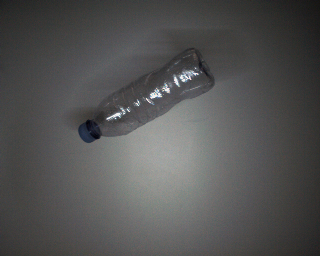
\includegraphics[width=\textwidth]{augmentation_brightness/1575026107_575_12_water-bottle_85}
    \caption{$B = 83$}
    \label{subfig:ab_85}
  \end{subfigure}
  \begin{subfigure}[b]{0.15\textwidth}
    \centering
    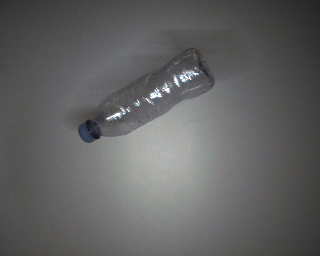
\includegraphics[width=\textwidth]{augmentation_brightness/1575026107_575_12_water-bottle_100}
    \caption{$B = 98$}
    \label{subfig:ab_100}
  \end{subfigure}
  \begin{subfigure}[b]{0.15\textwidth}
    \centering
    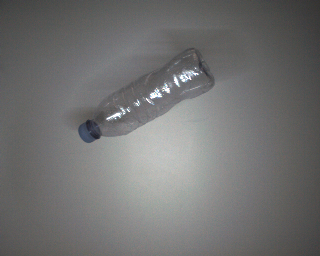
\includegraphics[width=\textwidth]{augmentation_brightness/1575026107_575_12_water-bottle_115}
    \caption{$B = 113$}
    \label{subfig:ab_115}
  \end{subfigure}
  \begin{subfigure}[b]{0.15\textwidth}
    \centering
    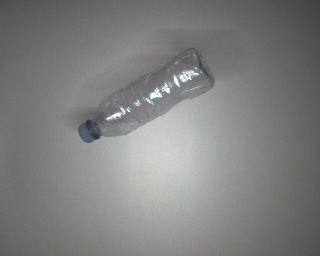
\includegraphics[width=\textwidth]{augmentation_brightness/1575026107_575_12_water-bottle_130}
    \caption{$B = 128$}
    \label{subfig:ab_130}
  \end{subfigure}
  \begin{subfigure}[b]{0.15\textwidth}
    \centering
    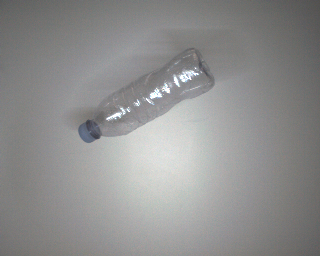
\includegraphics[width=\textwidth]{augmentation_brightness/1575026107_575_12_water-bottle_145}
    \caption{$B = 143$}
    \label{subfig:ab_145}
  \end{subfigure}
  \begin{subfigure}[b]{0.15\textwidth}
    \centering
    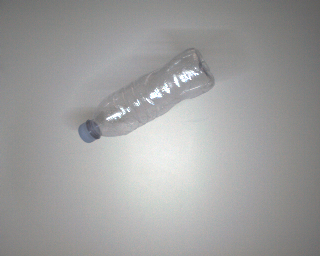
\includegraphics[width=\textwidth]{augmentation_brightness/1575026107_575_12_water-bottle_160}
    \caption{$B = 158$}
    \label{subfig:ab_160}
  \end{subfigure}
  \caption{Examples of resized frames of the \textit{Water Bottle}, where the brightness was adjusted according to the desired brightness levels}
  \label{fig:augmentation_brightness}
\end{figure}

% ------------------
\paragraph{Flipping}
Each frame is flipped vertically and horizontally to improve the orientation-independence of the objects in the frames.
Furthermore, the influence of the shadow that the object casts is decreased.
An example of these reflections is shown in figure \ref{fig:augmentation_flipping}.

The Python implementation uses the \acrshort{opencv} function \texttt{cv2.flip} to flip the frames around the x-axis (vertically) and around the y-axis (horizontally) \cite{training_opencv_flip}.

\begin{figure}
  \centering
  \begin{subfigure}[b]{0.3\textwidth}
    \centering
    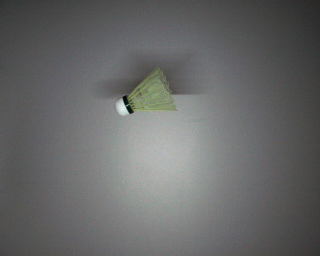
\includegraphics[width=\textwidth]{augmentation_flipping/1575023302_468_9_shuttlecock}
    \caption{Unaugmented}
    \label{subfig:af_resized}
  \end{subfigure}
  \begin{subfigure}[b]{0.3\textwidth}
    \centering
    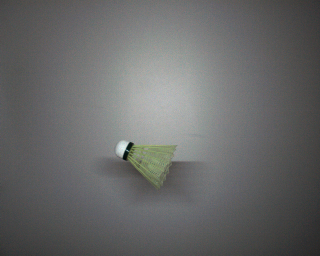
\includegraphics[width=\textwidth]{augmentation_flipping/1575023302_468_9_shuttlecock_v}
    \caption{Vertically flipped}
    \label{subfig:af_vertical}
  \end{subfigure}
  \begin{subfigure}[b]{0.3\textwidth}
    \centering
    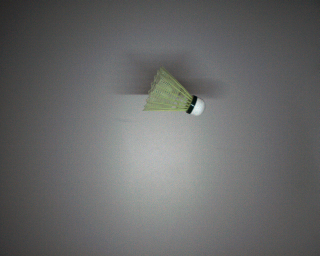
\includegraphics[width=\textwidth]{augmentation_flipping/1575023302_468_9_shuttlecock_h}
    \caption{Horizontally flipped}
    \label{subfig:af_horizontal}
  \end{subfigure}
  \caption{Example of a resized frame of the \textit{Shuttlecock} (\subref{subfig:af_resized}), which was flipped vertically (\subref{subfig:af_vertical}) and horizontally (\subref{subfig:af_horizontal})}
  \label{fig:augmentation_flipping}
\end{figure}

% ------------------------------------------------------------------------------------------------------------------------------
\subsection{Splitting}
\label{subsec:training_of_the_cnn:dataset:splitting}
During the fitting and evaluation process of the \acrshort{cnn} model, three splits of the dataset are required.
These required splits and their respective use is summarized in table \ref{tab:dataset_splits}.

\begin{table}
  \caption{Overview of the required dataset splits \cite{training_datasets}}
  \label{tab:dataset_splits}
  \centering
  \begin{tabular}{llp{10cm}}
    \toprule
    \textbf{Dataset} & \textbf{Split} & \textbf{Description} \\
    \midrule
    \textbf{Training} & \SI{70}{\percent} & The training split is used to fit the model. \\
    \midrule
    \textbf{Validation} & \SI{15}{\percent} & The validation split provides an evaluation of a model fit while tuning hyperparameters of the model. \\
    \midrule
    \textbf{Test} & \SI{15}{\percent} & The test split provides an unbiased evaluation of the final model fit (used to compare fit with other final models). \\
    \bottomrule
  \end{tabular}
\end{table}

It is crucial that the dataset splits are used in the right way.
For example, the validation and the test splits must never be used to fit the model.
Furthermore, it is important to know that the evaluation with the validation split becomes more biased as the classification performance is increased by tuning the hyperparameters of the model.
For this reason, a test split is used to evaluate and compare the final model fit.

The quantization process requires a small unlabeled dataset consisting of \numrange{100}{1000} frames for the calibration of the quantized model.
Seeing that the calibration of the quantized model has many similarities to the tuning of the hyperparameters, the required frames are chosen at random from the validation split.
In total, \num{990} frames are chosen from the validation split (largest possible multiple of the \num{22} classes).
The calibration dataset is thus a subset of the validation dataset without labels.

% ------------------------
\paragraph{Implementation}
The splitting of the dataset is implemented in the Python script \texttt{dataset\_generator.py}, which uses NumPy, \acrshort{opencv} and the standard library.

In a first step, the necessary information about the dataset is fetched from the \acrshort{mysql} database, which is used to store the labels, the file names and other useful metadata.
Table \ref{tab:tab_frames_structure} lists all columns of the database table \texttt{aionfpga.frames}.

\begin{table}
  \caption{Structure of the \acrshort{mysql} database table \texttt{aionfpga.frames}}
  \label{tab:tab_frames_structure}
  \centering
  \begin{tabular}{llll}
    \toprule
    \textbf{Column} & \textbf{Type} & \textbf{Length} & \textbf{Description} \\
    \midrule
    id & \texttt{INT} &  & Sequence number (unique identifier) \\
    timestamp & \texttt{INT} &  & The Unix timestamp at the time of the throw \\
    throwid & \texttt{INT} &  & Throw sequence number \\
    frameid & \texttt{INT} &  & Frame sequence number within a throw \\
    frame & \texttt{VARCHAR} & 255 & The file name of the frame \\
    object & \texttt{VARCHAR} & 255 & The name of the object in the frame (label) \\
    framegood & \texttt{INT} &  & \texttt{0}: frame unusable | \texttt{1}: frame usable \\
    partial & \texttt{INT} &  & \texttt{0}: object fully visible | \texttt{1}: object partially visible \\
    \bottomrule
  \end{tabular}
\end{table}

The slight imbalance in the dataset is mitigated in a next step.
There are several different methods to ensure that the dataset is balanced (e.g. collecting more data, resampling).
For the sake of simplicity, undersampling is used to remove samples from the overrepresented classes \cite{training_imbalanced}.

The actual implementation randomly selects frames from each class.
The number of selected frames is equal to the number of frames in the minority class.
The pseudorandom function used for the selection process is seeded to ensure repeatable results during different tests.
In this case, this results in a loss of about \SI{30.9}{\percent} of the collected frames.

In a third step, the data augmentation discussed in section \ref{subsec:training_of_the_cnn:dataset:augmentation} is performed.
The frames are first resized, then their brightness is adjusted and lastly they are flipped.
The brightness adjustment increases the size of the dataset by a factor of seven and the flipping by a factor of three.
This is due to the fact, that the original frames are preserved as well and results in a total increase of the dataset size by a factor of \num{21}.
Original refers in this case to the resized frames.

The next step is the actual splitting of the dataset.
For this purpose, the entire dataset is shuffled and then split according to table \ref{tab:dataset_splits}.

In a last step, the frames and the labels of the dataset splits are separately saved to the disk.
Due to the sheer number of frames in the dataset splits, the frames are saved in batches of \num{32}.
For this reason, \num{32} frames at a time are stored in a four-dimensional NumPy array of type \texttt{np.uint8} with a shape of $32\times 256\times 320\times 3$ (batch size $\times$ height $\times$ width $\times$ number of color channels).
The \num{22} different labels of the classes (object names) are mapped to a unique number between \num{0} and \num{21}.
This allows for an efficient way to store the labels in one-dimensional NumPy arrays of type \texttt{np.uint8}.
The length of these label arrays is determined by the number of frames in the respective splits.

For each split, both the batch arrays and the label array are saved to the disk in the binary NumPy (\texttt{.npy}) file format \cite{training_numpy_format}.
This allows for fast loading of the dataset from the disk \cite{training_numpy_npy}.

Listing \ref{lst:save_batches} shows the function \texttt{save\_batches}, which implements this last step.

\begin{lstlisting}[style=python, caption={Python function \texttt{save\_batches} to save the batch arrays and the label array}, label=lst:save_batches]
def save_batches(frames_name, labels_name, dst, frame_names, batch_size):

  num_frames = len(frame_names)
  num_batches = math.ceil(num_frames / batch_size)

  labels = np.empty((num_frames,), dtype=np.uint8)
  for idx in range(num_batches):
    start = idx * batch_size
    end = start + batch_size
    frame_names_slice = frame_names[start:end]

    frames = np.empty((len(frame_names_slice),) + fh.inf_shape, dtype=np.uint8)
    for i, frame in enumerate(frame_names_slice):
      obj_san = frame.split('_')[3]
      label = fh.objects_san.index(obj_san)
      frames[i] = cv2.imread(str(fh.dir_frames_augmented / f'{frame}.png'))
      labels[idx * batch_size + i] = label

    np.save(dst / f'{frames_name}_batch_{idx}_of_{num_batches}.npy', frames)

  np.save(dst / f'{labels_name}.npy', labels)
\end{lstlisting}

% ----------------
\paragraph{Result}
The toal number of frames after the augmentation is equal to \num{224070}.
The final training dataset consists of \num{156882} frames and requires \SI{35.91}{GiB} of disk space.
The validation and test datasets each comprise of \num{33594} frames and require \SI{15.38}{GiB} of disk space together.

\section{Architecture}
\label{sec:training_of_the_cnn:architecture}
% \todo[inline]{too much 'the', citations, todos, cleanup}

% Designing a \acrlong{cnn} architecture from scratch  (e.g. types and number of layers, number of filters, kernel size).
% The design of a \acrlong{cnn} architecture from scratch involves choosing the types of layers and their arrangement as well as many hyperparameters.
% Designing a \acrlong{cnn} architecture from scratch involves choosing the types of layers and their arrangement as well as many hyperparameters.
Designing a \acrlong{cnn} architecture from scratch requires choosing the types of layers and their arrangement as well as many hyperparameters.
% There are infinitely many ways to design a \acrlong{cnn} architecture from scratch (e.g. types of layers and their arrangement, many hyperparameters).
% There is currently no perfect way to design a good model and a lot of trial and error is 
For this reason, a lot of trial an error is involved in the design process of an adequate model \cite{training_arch_design}.
% For this reason, there are a infinitely many ways to design an adequate model and a lot of trial an error is involved in the design process of an adequate model. % todo: cite http://www.isikdogan.com/blog/how-to-design-a-convolutional-neural-network.html
There are, however, certain design principles that work really well \cite{training_arch_hyper}:
% the deeper in the net, the more filters and lower spatial dimensions (max pooling)

\begin{enumerate}
  % \item Starting with a low number of filters and increasing 
  \item Starting with a low number of filters (high-level feature detection)
  \item Increasing the number of filters towards the end (low-level feature detection)
  \item Decreasing the spatial dimensions of the feature maps towards the end
  \item Using kernel sizes of $3\times 3$, $5\times 5$ or $7\times 7$ for convolutional layers
  % \item Using kernel sizes of $2\times 2$ or $3\times 3$ with a stride of two for max-pooling layers
  \item Using pool sizes of $2\times 2$ or $3\times 3$ with a stride of two for max-pooling layers
  \item Adding additional layers until the model is overfitting
  \item Using state-of-the-art networks as inspiration
\end{enumerate}

% A summary of all the layers is listed in table \ref{tab:arch}.
A summary of all the layers of the final \acrshort{cnn} architecture is listed in table \ref{tab:arch}.
% A kernel size of $5\times 5$ is chosen for the first convolutional layer
% Due to the large input shape of the frames, a larger kernel size of $5\times 5$ is chosen for the first convolutional layer.
% The first convolutional layer uses \num{16} filters and a larger kernel size of $5\times 5$ due to the large input shape of the frames.
The first convolutional layer uses only \num{16} filters and a larger kernel size of $5\times 5$ due to the large dimensions of the input images.
All other convolutional layers use a kernel size of $3\times 3$ while steadily increasing the number of used filters up to \num{128}.
% only max pooling is used
% max amount of poooling layers used (iage size of 5x4)
% The architecture uses the maximum amount of max-pooling layers for the given input shape.
% The designed architecture uses six max-pooling layers with a kernel size of $2\times 2$ and a stride of two.
The designed architecture uses six max-pooling layers with a pool size of $2\times 2$ and a stride of two.
% This reduces the spatial dimensions of the input feature maps down to $4\times 5$.
This reduces the spatial dimensions of the feature maps to $4\times 5$ (height $\times$ width).
% The fully-connected layer \texttt{fc8} is several times larger than the output layer \texttt{fc9}.
The output of the fully-connected layer \texttt{fc8} is about the size of the output layer \texttt{fc9} squared.
This allows the output layer to combine many of the different high-level features to create a confident prediction.
% This allows the output layer a variety of combinations of the different high-level features 

% no more layers were added (was simply not necessary, it converged incredible fast)
Even though the model was not yet overfitting, no additional layers were added.
% The reason for this is that the classification performance is already exceptional with the current architecture.
% The reason for this is that with the current architecture the classification performance is already exceptional (see section \ref{sec:training_of_the_cnn:training}).
The reason for this is that with the current architecture the classification performance is already exceptional.

% number of parameter relatively low compared to state-of-the-art networks
% compare this and back up with the citation below
% Furthermore, the number of trainable parameters (weights) is relative low compared to state-of-the-art networks (e.g. VGG, ResNet, Inception) \cite{}. % todo: cite https://keras.io/api/applications/
Furthermore, the number of trainable parameters (weights) is relative low compared to state-of-the-art networks like VGG, ResNet or Inception \cite{training_arch_keras}.
This increases the throughput considerably, as less mathematical operations are required.
% talk about the importance of keeping the parameters of the first fc layer down!
% The keys to keeping the total number of trainable parameter low are the shape of the feature maps of the last convolutional layer and the artifical output neurons of the first dense layer.
% This is evident when analyzing the number of trainable parameters listed in table \ref{tab:arch}.
The key to keeping the total number of trainable parameter low is evident when analyzing table \ref{tab:arch}.
% A whopping \num{1311232} of the \num{1614486} total weights stem from the connection between those layers.
% A whopping \num{1311232} of the \num{1614486} total weights can be attributed to the connection between these layers.
A whopping \num{1311232} of the \num{1614486} total weights can be attributed to the connection between the feature maps of the last convolutional layer \texttt{conv7} and the artificial output neurons of the first dense layer \texttt{fc8}.
This accounts for \SI{81.22}{\percent} of all trainable parameters.
% This is the reason why the spatial dimensions of the feature maps should be decreased towards the end.
For this reason the spatial dimensions of the feature maps should be decreased towards the end.
% For this reason the spatial dimensions of the feature maps should decrease towards the end. % todo: maybe use this?

\begin{table}
  \caption{Layers of the \acrshort{cnn} architecture}
  \label{tab:arch}
  \centering
  \begin{tabular}{lllllll}
    \toprule
    \textbf{Layer} & \textbf{Type} & \textbf{Activation} & \textbf{Filters} & \textbf{Kernel} & \textbf{Output Shape} & \textbf{Param \#} \\
    \midrule
    \textbf{conv1} & \texttt{Conv2D} & \acrshort{relu} & \num{16} & $5\times 5$ & $256\times 320\times 16$ & \num{1216} \\
    \textbf{pool1} & \texttt{MaxPooling2D} &  &  & $2\times 2$ & $128\times 160\times 16$ & \num{0} \\
    \midrule
    \textbf{conv2} & \texttt{Conv2D} & \acrshort{relu} & \num{32} & $3\times 3$ & $128\times 160\times 32$ & \num{4640} \\
    \textbf{pool2} & \texttt{MaxPooling2D} &  &  & $2\times 2$ & $64\times 80\times 32$ & \num{0} \\
    \midrule
    \textbf{conv3} & \texttt{Conv2D} & \acrshort{relu} & \num{32} & $3\times 3$ & $64\times 80\times 32$ & \num{9248} \\
    \textbf{pool3} & \texttt{MaxPooling2D} &  &  & $2\times 2$ & $32\times 40\times 32$ & \num{0} \\
    \midrule
    \textbf{conv4} & \texttt{Conv2D} & \acrshort{relu} & \num{64} & $3\times 3$ & $32\times 40\times 64$ & \num{18496} \\
    \textbf{pool4} & \texttt{MaxPooling2D} &  &  & $2\times 2$ & $16\times 20\times 64$ & \num{0} \\
    \midrule
    \textbf{conv5} & \texttt{Conv2D} & \acrshort{relu} & \num{64} & $3\times 3$ & $16\times 20\times 64$ & \num{36928} \\
    \textbf{pool5} & \texttt{MaxPooling2D} &  &  & $2\times 2$ & $8\times 10\times 64$ & \num{0} \\
    \midrule
    \textbf{conv6} & \texttt{Conv2D} & \acrshort{relu} & \num{128} & $3\times 3$ & $8\times 10\times 128$ & \num{73856} \\
    \textbf{pool6} & \texttt{MaxPooling2D} &  &  & $2\times 2$ & $4\times 5\times 128$ & \num{0} \\
    \midrule
    \textbf{conv7} & \texttt{Conv2D} & \acrshort{relu} & \num{128} & $3\times 3$ & $4\times 5\times 128$ & \num{147584} \\
    \midrule
    \textbf{flatten} & \texttt{Flatten} &  &  &  & \num{2560} & \num{0} \\
    \textbf{fc8} & \texttt{Dense} & \acrshort{relu} &  &  & \num{512} & \num{1311232} \\
    \textbf{fc9} & \texttt{Dense} &  &  &  & \num{22} & \num{11286} \\
    \bottomrule
  \end{tabular}
\end{table}

\subsection{Visualization}
\label{subsec:training_of_the_cnn:architecture:visualization}
% The final architecture of the \acrshort{cnn} model is visualized in figure \ref{fig:arch}.
% Figure \ref{fig:arch} shows the final architecture of the \acrshort{cnn} model.
% Figure \ref{fig:arch} visualizes the final architecture of the \acrshort{cnn} model listed in table \ref{tab:arch}.
Figure \ref{fig:arch} visualizes the final architecture of the \acrshort{cnn} model.
The visualization was created with Ti\textit{k}Z and the help of the open-source repository \textit{PlotNeuralNetwork} \cite{training_arch_plot}.
% The final architecture of the \acrshort{cnn} model shown in figure \ref{fig:arch} was visualized with the help of the open source tool PlotNeuralNetwork \cite{}.
% todo: cite https://github.com/HarisIqbal88/PlotNeuralNet or https://doi.org/10.5281/zenodo.2526396
% Haris Iqbal. (2018, December 25). HarisIqbal88/PlotNeuralNet v1.0.0 (Version v1.0.0). Zenodo. http://doi.org/10.5281/zenodo.2526396

% todo: lots of sentences starting with 'the'
The boxes represent the outputs of the different layers.
% The light orange boxes with darker orange bands represent convolutional layers with the \acrshort{relu} activation function.
% The light orange boxes with darker orange bands represent convolutional layers, which use the \acrshort{relu} activation function.
% The light orange boxes with darker orange bands represent the feature maps of the convolutional layers, which use the \acrshort{relu} activation function.
% The light orange boxes with darker orange bands represent the feature maps of the convolutional layers with the \acrshort{relu} activation function applied.
% The light orange boxes represent the feature maps of the convolutional layers and the darker orange bands indicate that the \acrshort{relu} activation function is applied.
On the one hand, the light orange boxes represent the feature maps of the convolutional layers and, on the other hand the purple boxes represent the artificial output neurons of the dense layers.
The darker colored bands on the boxes indicate that the \acrshort{relu} activation function is applied.
% darker orange bands indicate that the \acrshort{relu} activation function is applied.
% Again, the darker purple band of \texttt{fc8} indicates that the \acrshort{relu} activation function is applied
The red boxes represent max-pooling layers, which decrease the spatial dimensions.
% The dashed lines between the output of \texttt{conv7} and \texttt{fc8} depict the flattening and the dense connection between of the convolutional layer
% The dashed lines between the output of \texttt{conv7} and \texttt{fc8} depict the flattening as well as the dense connection between the layer outputs.
% The dashed lines between the output of \texttt{conv7} and \texttt{fc8} depict the flattening as well as the dense connection.
The dashed lines between the output of \texttt{conv7} and \texttt{fc8} depict the flattening in addition to the dense connection.

\begin{figure}
  \centering
  \includegraphics[width=\textwidth]{arch}
  \caption{Final architecture of the \acrlong{cnn}}
  \label{fig:arch}
\end{figure}

\subsection{Implementation}
\label{subsec:training_of_the_cnn:architecture:implementation}
% The dataset augmentation is done with the Python script \texttt{dataset\_generator.py}, which uses NumPy as well as the Python implementation of the \acrfull{opencv}.
% The \acrshort{cnn} architecture is implemented in the Python script \texttt{cnn.py}, as shown in listing \ref{lst:arch}.
The \acrshort{cnn} architecture is defined in the Python script \texttt{cnn.py}, as shown in listing \ref{lst:arch}.
% implementation with TF 2.2.0, Keras backend/frontend?!, PYthon
% Implementation of the Keras API meant to be a high-level API for TensorFlow.
% The script uses the open-source software library TensorFlow v2.2.0, which serves as the default backend for Keras
% The script uses the open-source software library TensorFlow v2.2.0, along with the high-level Keras \acrshort{api} in the \texttt{tf.keras} module \cite{}. % todo: cite https://www.tensorflow.org/versions/r2.2/api_docs/python/tf/keras
The script uses the open-source software library TensorFlow v2.2.0, along with the high-level Keras \acrshort{api} implemented in the \texttt{tf.keras} module \cite{training_arch_tf_keras}.
% todo: or maybe cite https://www.tensorflow.org/api_docs/python/tf/keras
% easy implementation with the sequential model
To define the architecture a \texttt{Sequential} model is used to arrange the desired layers in a plain stack \cite{training_arch_tf_keras_seq}.

\begin{lstlisting}[style=python, caption={Sequential model}, label=lst:arch]
# Convolutional Neural Network Architecture
# Convolution layers
model = models.Sequential()
model.add(layers.Conv2D(16, (5, 5), padding='same', activation='relu', input_shape=fh.inf_shape))
model.add(layers.MaxPooling2D((2, 2)))
model.add(layers.Conv2D(32, (3, 3), padding='same', activation='relu'))
model.add(layers.MaxPooling2D((2, 2)))
model.add(layers.Conv2D(32, (3, 3), padding='same', activation='relu'))
model.add(layers.MaxPooling2D((2, 2)))
model.add(layers.Conv2D(64, (3, 3), padding='same', activation='relu'))
model.add(layers.MaxPooling2D((2, 2)))
model.add(layers.Conv2D(64, (3, 3), padding='same', activation='relu'))
model.add(layers.MaxPooling2D((2, 2)))
model.add(layers.Conv2D(128, (3, 3), padding='same', activation='relu'))
model.add(layers.MaxPooling2D((2, 2)))
model.add(layers.Conv2D(128, (3, 3), padding='same', activation='relu'))

# Dense layers
model.add(layers.Flatten())
model.add(layers.Dense(512, activation='relu'))
model.add(layers.Dense(22))
\end{lstlisting}

\section{Training}
\label{sec:training}




\chapter{Hardware}
\label{ch:hardware}

\section{Throwing Booth}
\label{sec:hardware:throwing_booth}

The booth is constructed from Item aluminum profiles.
The background of the images shall remain the same, regardless of the current location.
Therefore, a white side wall opposite the camera is used.
When creating the booth design, care was taken to ensure that the size corresponds to the width of a table (\SI{750}{mm}).

The objects should be thrown as far away from the camera as possible to be able to take more pictures per throw.
To ensure that the objects are thrown through the field of view and as far away from the camera as possible, there is a hole in the rear wall as a target.
It is located on the right side of the rear wall, which is further away from the camera.
If the objects are shot through the hole in the rear wall, they end up in a net.

The rear panel is made of a \SI{5}{mm} thick ABS plate.
This material is robust and withstands the impacts of the throwing objects.
The side wall is made of foamed PVC.
Due to the manufacturing process, the plate is less smooth, which results in less light reflections and therefore better pictures.

The whole throwing booth is drawn in the CAD tool Inventor. It is designed with all its components using a 3D model.
The camera is mounted on an Item profile with an aluminum mounting adapter and protected from damage with an aluminum sheet.
Both components have slotted holes to allow fine adjustments during assembly.
Figure \ref{fig:booth} shows a 3D model of the throwing booth. 

\begin{figure}[h]
	\centering
	\includegraphics[width=0.5\textwidth]{graphics/top_assembly.png}
	\caption{3D model of the throwing booth}
	\label{fig:booth}
\end{figure}

\section{Case}
\label{sec:hardware:case}

The power supplies for all electronic components are placed in a box together with the Ultra96-V2.
The box is a case from Fibox with a transparent cover to give visitors an impression of the way it works.
It features a \SI{230}{VAC} power cable, a \SI{24}{VDC} output for lighting, a Mini DisplayPort cable for the monitor and the USB cable for the camera.
In addition, there are three fans on the walls to ensure that the Ultra96-V2 and the power supply is cooled.
The box also contains terminal blocks and cable trunking to store cables that are too long.
All components are mounted on a metal plate.
Figure \ref{fig:fibox3d} shows a 3D model of the box. 

\begin{figure}[h]
	\centering
	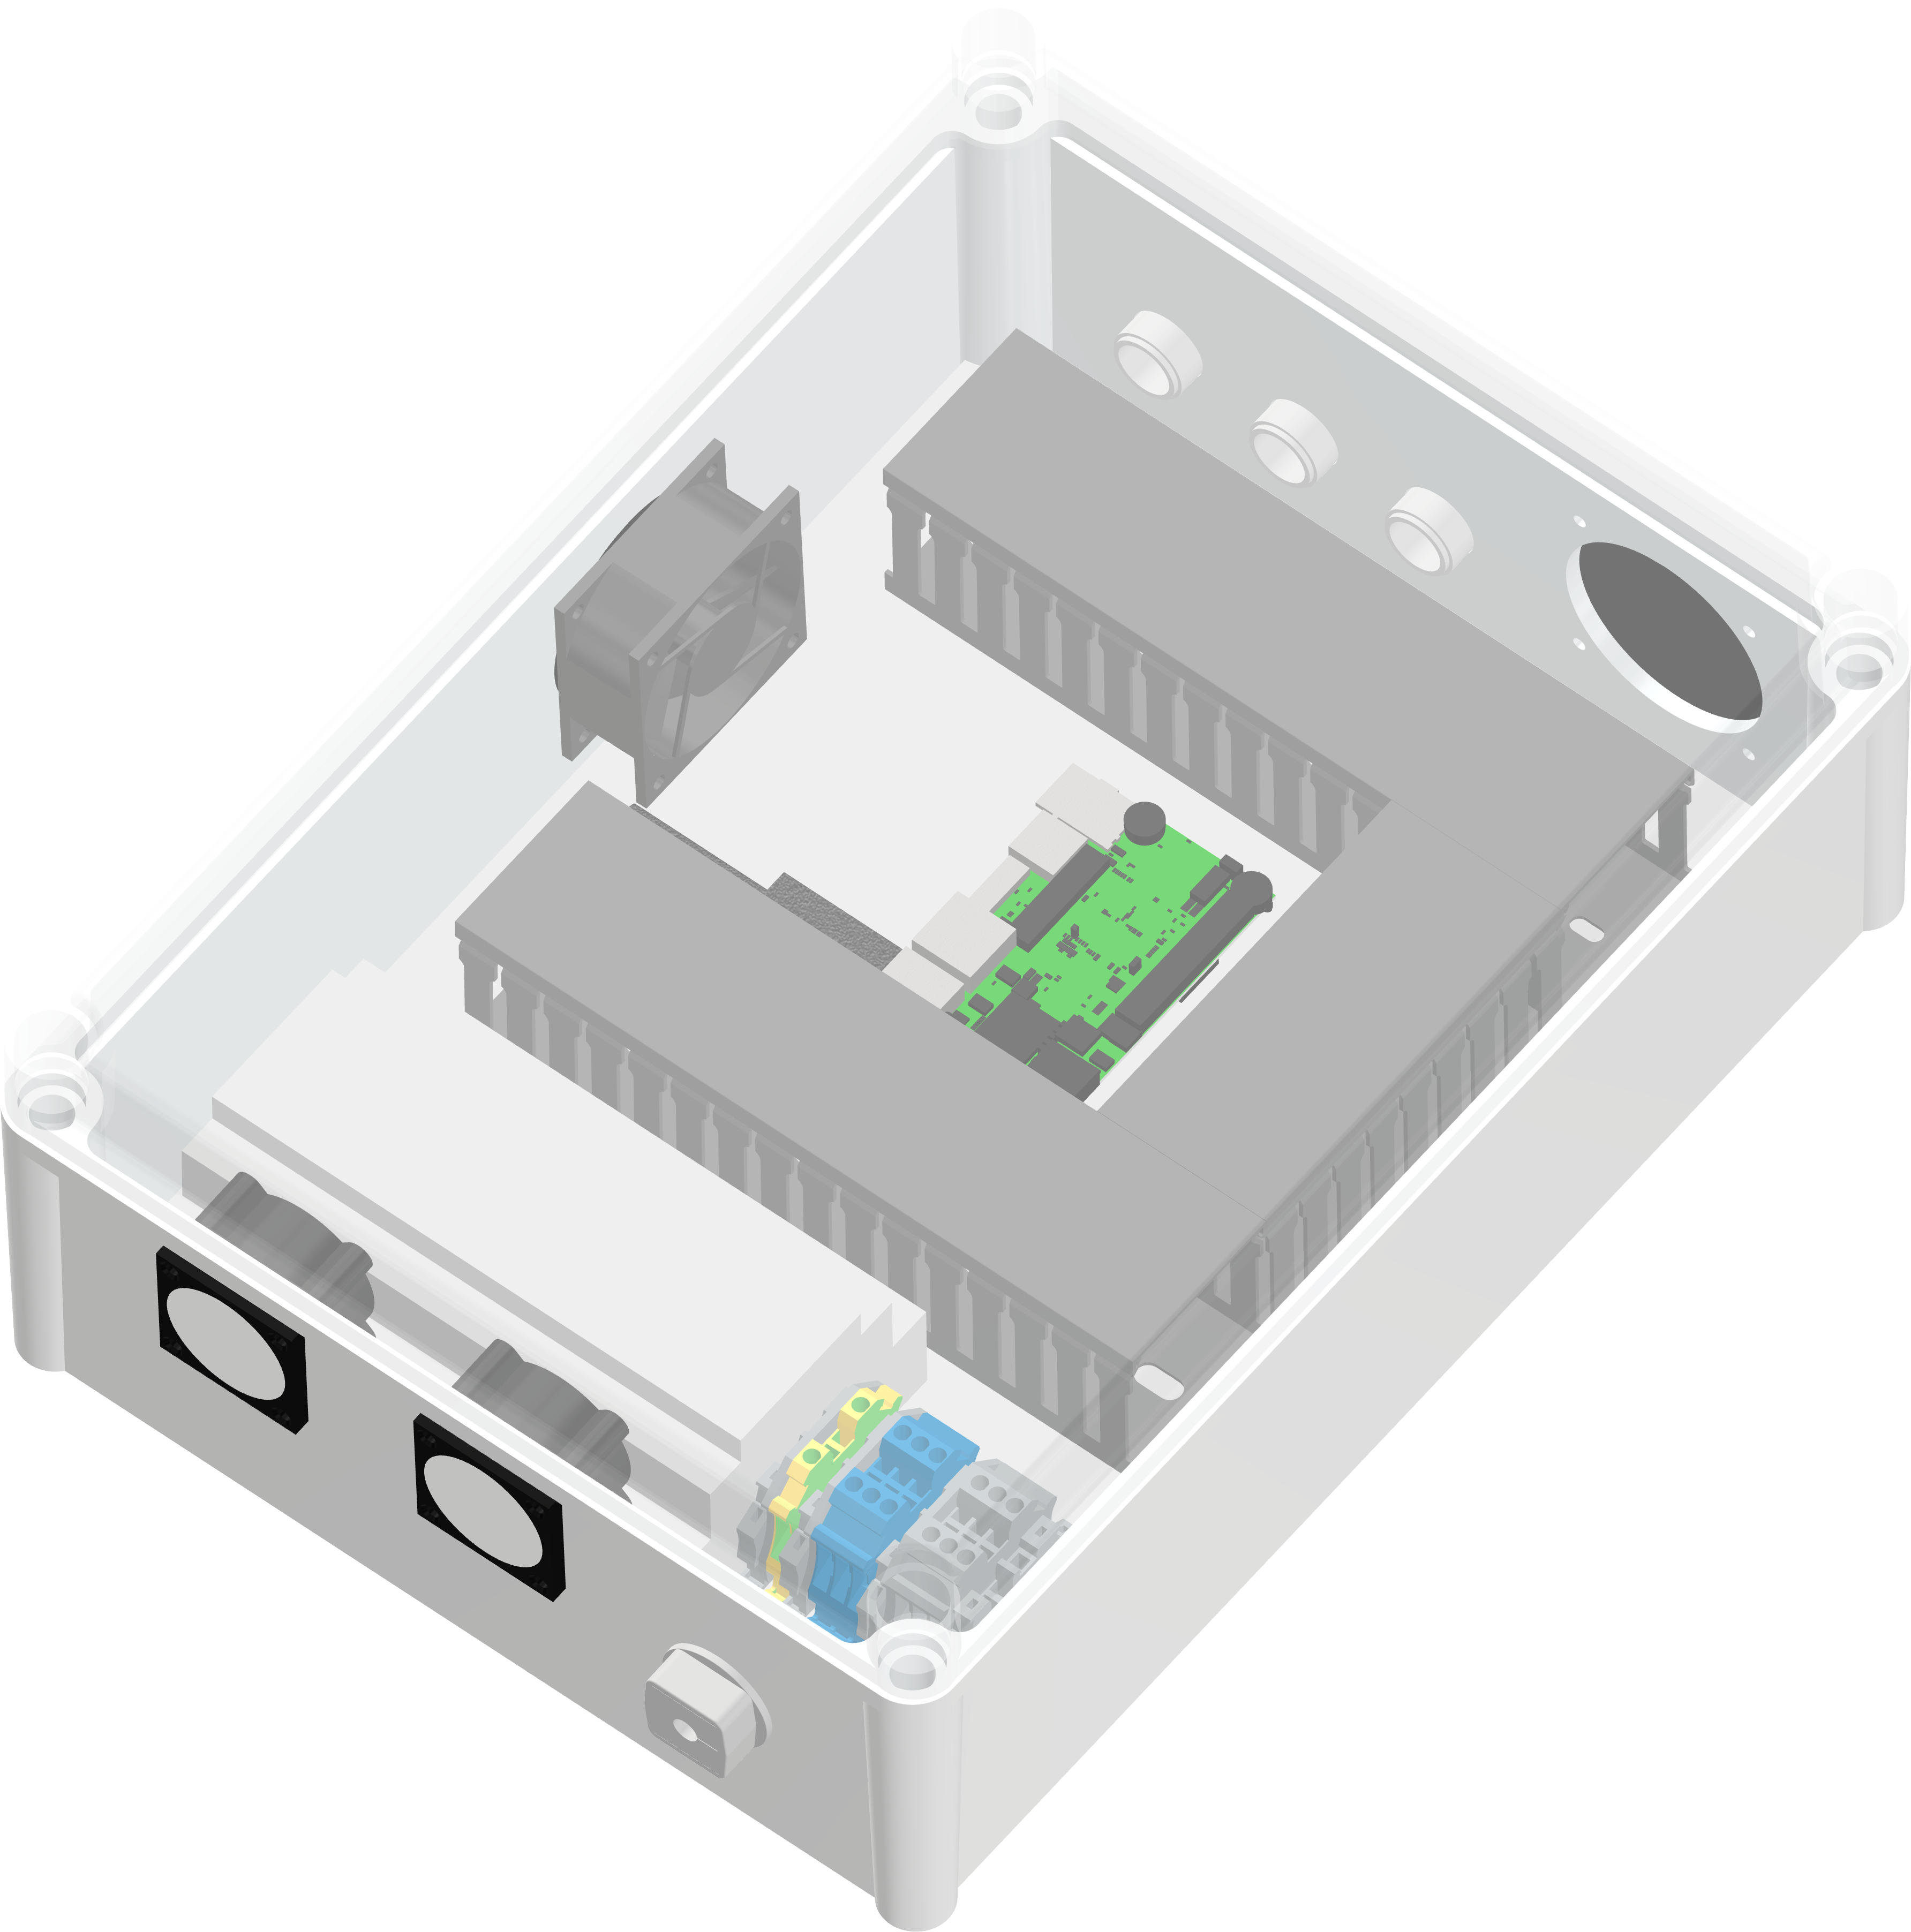
\includegraphics[width=0.5\textwidth]{graphics/case.png}
	\caption{3D model of the Fibox case}
	\label{fig:fibox3d}
\end{figure}

\section{Camera}
\label{sec:hardware:camera}

In this project a VCXU-13C industrial camera from Baumer is used.
The Baumer company produces various sensors, such as CMOS sensors with different specifications.
The VCXU-13C camera features a global shutter.
Furthermore, it has a USB 3.0 interface for data transfer.
This is necessary because the Ultra96-V2 has no Ethernet interface.
The maximum frame rate of the camera is \SI{222}{fps}, which guarantees at least three pictures per throw.
The minimum exposure time is \SI{20}{\micro s} \cite{baumer_cam}.

The industrial camera requires a lens for proper operation.
Suitable for the camera is the lens ZVL-FL-HC0614-2M, which is also manufactured by Baumer.
The aperture is operated manually to focus the images.

\section{Lighting}
\label{sec:hardware:lighting}

The more light there is, the shorter the exposure time can be selected.
This results in a clearer image, which is an advantage in image recognition.
In order for the objects to be as independent as possible from the lighting, the lighting must not flicker and the field of view should be illuminated as uniformly as possible.
Therefore, diffuse lighting is required.
The SVL BAR LIGHT LHF300-WHI from Stemmer Imaging is used because it meets these requirements.

\section{MPSoC Development Board}
\label{sec:hardware:mpsoc_development_board}

The hardware is an Ultra96-V2 board, which is distributed by Avnet.
The \acrfull{mpsoc} placed on it is a Xilinx Zynq UltraScale+ \acrshort{mpsoc} ZU3EG.
This chip is from the Zynq UltraScale+ family and has an UltraScale architecture.
Integrated is a quad-core ARM Cortex A53 processor to run a complete operating system and a dual-core ARM Cortex R5, which makes the Ultra96-V2 hard real-time capable.
The A53 core can be clocked with \SI{1.5}{GHz}, the R5 with \SI{600}{MHz}.

The \acrshort{fpga} on the \acrshort{mpsoc} allows a hardware acceleration of up to a factor of 20 compared to the fastest CPUs \cite{acceleration_xilinx}.
Avnet therefore recommends the board as ideal for the field of high-speed artificial intelligence \cite{ai_resources_xilinx}.
The most important specifications of the \acrshort{mpsoc} are listed in the following table \ref{tab:specs_MPSoC}.

\begin{table}[h]
	\caption{Xilinx Zynq UltraScale+ \acrshort{mpsoc} ZU3EG key features \cite{xilinx_zynq}}
	\label{tab:specs_MPSoC}
	\centering
	\begin{tabular}{ll}
		\toprule
		& \textbf{ZU3EG} \\
		\midrule
		\textbf{Logic Cells} & \SI{154}{k} \\
		\textbf{Flip Flops} & \SI{141}{k} \\
		\textbf{\acrshort{bram}} & \SI{7.6}{Mb} \\
		\textbf{\acrshort{dsp} Slices} & 360 \\
		\bottomrule
	\end{tabular}
\end{table}

The Ultra96-V2 also features two USB 3.0 ports and \SI{2}{GB} \acrfull{lpddr4} \acrshort{ram}, which are essential for fast image processing.
A \acrfull{mdp} serves as a connection to a monitor \cite{avnet_ultra96v2}.
This guarantees a standalone operation.



\chapter{Embedded Platform}
\label{ch:embedded_platform}

\section{MPSoC Block Diagram}
\label{sec:embedded_platform:block_diagram}

Figure \ref{fig:hardware_overview} shows the most important hardware components for this project on the Ultra96-V2 board.
Communication and data transfer is handled by the interconnects, on the \acrlong{pl} side it is the AXI Interconnect \cite{mpsoc_memory}.
Recorded frames are stored in the \acrshort{ram} and retrieved when needed.
The Mali-400 MP2 is an OpenGL multi core \acrfull{gpu} distributed by ARM \cite{arm_mali}.
A \acrshort{gpu} is required to use the graphical interface.
The \acrshort{pl} contains the \acrshort{dpu} to run inference.
The application and the operating system run on the ARM processor.

\begin{figure}
  \centering
  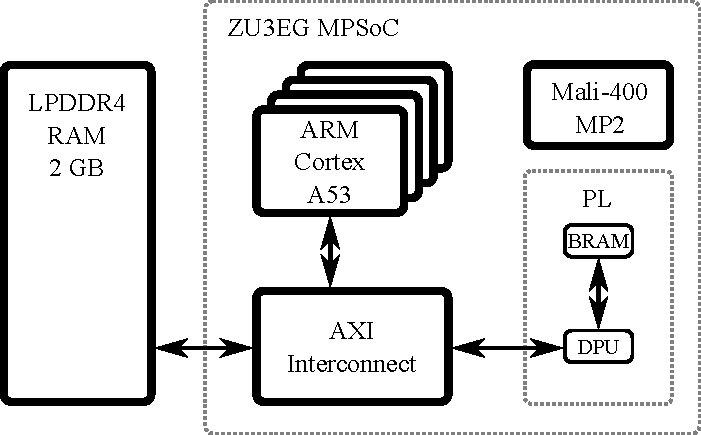
\includegraphics[width=0.5\textwidth]{graphics/hardware_overview.pdf}
  \caption{Available hardware on the Ultra96-V2}
  \label{fig:hardware_overview}
\end{figure}

\section{Host Prerequisites}
\label{sec:embedded_platform:host_prerequisites}
\todo[inline]{all}

\subsection{Hardware Prerequisites}
\label{subsec:embedded_platform:host_prerequisites:hardware_prerequisites}

\subsection{Xilinx Tools}
\label{subsec:embedded_platform:host_prerequisites:xilinx_tools}
% Short intro, how Xilinx works with Vivado, Vitis and Vitis AI.
% Explain, which tools were used, also explain requirements host and other installed tools (bsp docker)
The Xilinx tools are not added to the path while installing.
Therefore, a shell script, located in the installation directory needs to be sourced.
For Petalinux, it could look like this:
\begin{lstlisting}[style=bash, caption={}, label=lst:]
  source /opt/xilinx/petalinux/2019.2/settings.sh
\end{lstlisting}
% Install in default location, because of hardcoded paths.
% Petalinux using yocto

\section{Xilinx Tools}
\label{sec:embedded_platform:xilinx_tools}

\paragraph{PetaLinux}
PetaLinux is an embedded Linux \acrfull{sdk}.
It is a development tool that contains everything necessary to build, develop, test, and deploy embedded Linux systems.
In the background PetaLinux is running Yocto functions.
The goal of PetaLinux is to make it easier for developers to build an own embedded Linux \cite{petalinux_user_guide}.

\paragraph{Vivado}
Xilinx offers many tools to work with their hardware.
The traditional way is to design hardware with a \acrfull{hdl} like VHDL or Verilog.
These \acrfull{rtl} descriptions are passed to a synthesis tool and written to the \acrshort{fpga}.
% This functionality is embraced by the Vivado Design Suite HLx Editions.
This functionality is provided by the Vivado Design Suite HLx editions.
The output of Vivado is a bitstream that can be loaded to the target \cite{vivado_user_guide}.

\paragraph{Vitis Unified Software Platform}
% Vitis Unified Software Platform in short sometimes called Vitis provides software developers with the ability to build accelerated applications.
Vitis Unified Software Platform, or Vitis for short, offers software developers the ability to build accelerated applications.
% To communicate with the hardware \acrfullpl{api} are used.
\Acrfullpl{api} are used to communicate with the hardware.
% The Vitis core development kit includes the v++ compiler for the hardware kernel, the g++ compiler for compiling the application to run on an x86 host, and an ARM compiler for cross-compiling the application to run on the embedded processor of a Xilinx device \cite{vitis_user_guide}.
The Vitis core development kit includes the v++ compiler for the hardware kernel and the g++ compiler for compiling the application to run on an x86 host.
It also includes an ARM compiler for cross-compiling the application to run on the embedded processor of a Xilinx device \cite{vitis_user_guide}.

\paragraph{Vitis AI}
The Vitis AI development environment consists of the Vitis AI development kit.
It contains an AI compiler, an AI quantizer, an AI optimizer as well as the libraries to run inference and the \acrfull{xrt}.
Example designs are also included.
AI inference on Edge devices and Alveo accelerator cards are available with Vitis AI \cite{vitis_ai_user_guide}.
Vitis AI replaces the old \acrshort{dnndk} toolchain since version 2019.2.

\paragraph{Acceleration Runtime}
% In the \acrfull{xrt} a combination of userspace and kernel driver components are included.
The \acrfull{xrt} contains a combination of user space and kernel driver components.
% The advantage of the \acrshort{xrt} for the user is that there is very little porting effort when migrating an application from PCIe based platforms to MPSoC based edge platforms or from one edge platform to another.
The advantage of the \acrshort{xrt} for the user is that when migrating an application from PCIe-based platforms to MPSoC-based edge platforms or from one edge platform to another, there is very little porting effort.
When working with Vitis AI, it handles the \acrshort{xrt} in the background \cite{xrt_overview}.

\paragraph{Neural Network Runtime}
\acrshort{n2cube} is based on the \acrshort{xrt}.
It provides the \acrshortpl{api} to develop an \acrshort{ai} application in Python or C++ \cite{vitis_ai_user_guide}.

\paragraph{Versions}
Xilinx releases two to three versions per year.
% These follow the naming scheme, that first the year is written and then a number, which starts at 1 and is incremented for every new version.
These follow the naming scheme that the year is written first and then a number starting at 1, which is incremented with each new version.
It is important to use the same version for PetaLinux, \acrshort{xrt} and Vitis.
Vitis was first released in version 2019.2.

\paragraph{Using Xilinx Tools}
% While installing Vitis, Vivado is installed as well by default.
When Vitis is installed, Vivado is also installed by default.
The Xilinx tools are not added to the path when installed.
% Therefore, a shell script, located in the installation directory needs to be sourced.
Therefore, a shell script, which is located in the installation directory, must be sourced.
For example, sourcing PetaLinux could look like this:
\begin{lstlisting}[style=bash, caption={}, label=lst:source_tools]
  source /tools/petalinux/2019.2/settings.sh
\end{lstlisting}
% Avnet expects that the user installs the tools in the default install directory.
Avnet expects the user to install the tools in the default installation directory.
For Vitis the default directory is \texttt{/tools/Xilinx/} and for PetaLinux it is \texttt{/tools/}.
To avoid problems, it is recommended not to change the default directories.
% Install in default location, because of hardcoded paths.

\section{Operating Systems}
\label{sec:embedded_platform:operating_systems}
In the following chapter two possible operating systems will be considered.
On one side, this is an operating system which can be built with Petalinux Tools.
On the other side, there is PYNQ.

\subsection{PetaLinux}
\label{subsec:embedded_platform:operating_systems:petalinux}

Xilinx provides PetaLinux Tools to build your own PetaLinux \acrshort{os}.
It is recommended to work with the so-called target platform.
The target platform is a combination of hardware and software components.
The most important hardware component is a proprietary file format, called XSA.
XSA stands for Xilinx Support Archive and contains one or more \texttt{.hwh} files, \texttt{.bit} files, driver files and other metadata files.
A hardware hand-off file (\texttt{.hwh} file) stores information about the Vivado tool version and the board tag.
Furthermore, \texttt{.hwh} files contain \acrshort{ip} instances, name and parameters as well as memory map information of the processors \cite{vitis_user_guide}.

It is also possible to download the pre-built platform from Element14.
However, to customize the working environment, it is necessary to build the platform by hand.
Avnet provides all files for the Ultra96-V2 board via GitHub to build a custom target platform.

\paragraph{Development Flow}
Figure \ref{fig:petalinux_workflow} shows the workflow graphically.
Red names mean that the files on the SD card are needed, while black names serve as intermediate files to create additional red files.
The grayed out field needs further programs from Xilinx to be executed.
This step is not essential, but can improve performance.
It is not used in this project, however.
The Vitis Platform step is described in more detail in the following sections.
Building the \acrshort{dpu} is described in section \ref{sec:embedded_platform:dpu}, and the model deployment procedure is documented in section \ref{sec:embedded_platform:model_deployment}.

\begin{figure}
  \centering
  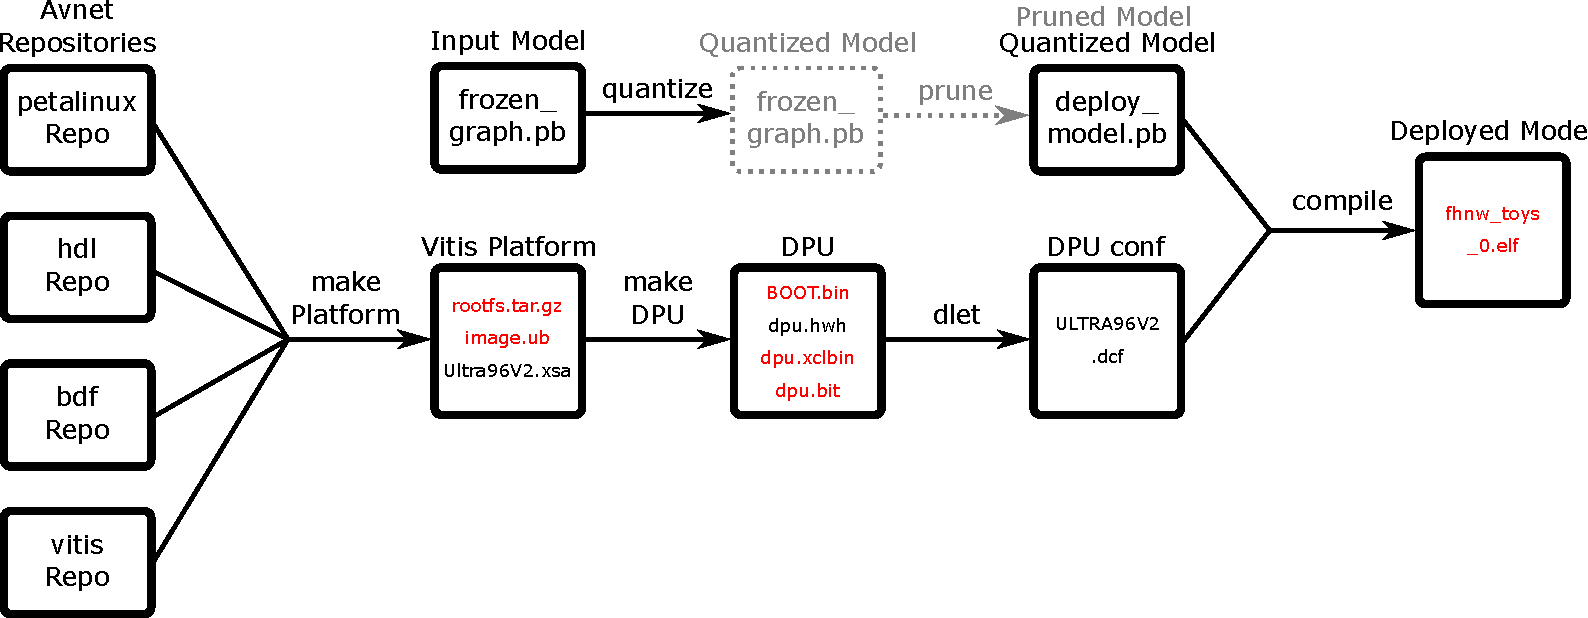
\includegraphics[width=1\textwidth]{graphics/workflow.pdf}
  \caption{PetaLinux workflow}
  \label{fig:petalinux_workflow}
\end{figure}

\paragraph{Build own Vitis Platform}
Four repositories from Avnet are required:
\begin{itemize}
  \item \texttt{bdf}
  \item \texttt{hdl}
  \item \texttt{petalinux}
  \item \texttt{vitis}
\end{itemize}

The \texttt{bdf} (board definition files) repository contains one folder for each of their development boards.
The \texttt{hdl} repo is required to use the \acrfull{pl} on UltraScale+ \acrshortpl{mpsoc}.
The \texttt{petalinux} archive contains, among other things, the configurations of the operating system PetaLinux.
To build a Vitis platform, the \texttt{vitis} archive is also required.
The \texttt{vitis} folder contains several Makefiles which refer to the other three repositories.
The repositories \texttt{hdl} and \texttt{petalinux} must be checked out to the same branch as the Xilinx Tools version.

The building process can be started with the Makefile in the \texttt{vitis/} directory.
Which board is used must be specified as a parameter.
Building the platform takes several hours, requires about \SI{200}{GB} of disk space and a minimum of \SI{32}{GB} of RAM.
After the process is completed, the platform is located in the \texttt{vitis/platform\_repo/} directory.

The Makefile from Avnet creates a sysroot by default.
Since all header and library files are included in this directory structure, cross compiling an application is possible.

\paragraph{Configure own Vitis Platform}
The platform can be adapted to individual needs.
First, a new PetaLinux project is created.
The generated directory \texttt{project-spec/meta-user} contains recipes for adding or removing programs like \acrshort{opencv} or a package manager.
Own recipes can be created with the command \texttt{petalinux-create -t apps}.
It is possible to create a component from existing content or from a predefined application template \cite{petalinux_commandline_guide}.

After adding all recipes, the commands \texttt{petalinux-config} and \texttt{petalinux-build} create the custom root filesystem, the required boot files and the Linux kernel \cite{petalinux_user_guide}.

The first stage bootloader, the device tree blob and U-Boot are stored in the \texttt{BOOT.BIN} file by default configuration.
They are required to initialize the board and load the kernel image \cite{xilinx_wiki_boot}.
The kernel image is located in the \texttt{image.ub} file \cite{xilinx_wiki_uboot}.
Both files are located in the \texttt{petalinux/projects/ultra96v2\_oob\_2019\_2/images/linux/} directory.

\paragraph{Flash SD Card}
The first step is to create the partitions for the boot files and for the root filesystem.
For the boot partition the format should be FAT32, while the root filesystem partition should be Ext4.
A space of \SI{1}{GB} for the boot partition is sufficient.
Furthermore, the boot label should be set for the boot partition.
In a next step, the created partitions must be formatted.
In a shell script it can be done as follows:

\begin{lstlisting}[style=bash, caption={Prepare SD card}, label=lst:create_partitions]
  DISK=/dev/sdb
  PART=

  # Create partitions
  sudo parted $DISK -s mkpart primary fat32 1MiB 1025MiB
  sudo parted $DISK -s mkpart primary ext4 1026MiB 100%

  # Set boot label
  sudo parted $DISK -s set 1 boot on

  # format partitions
  sudo mkfs -t vfat -F 32 -n boot $DISK${PART}1
  sudo mkfs -t ext4 -L rootfs $DISK${PART}2
\end{lstlisting}

The SD card is now ready to save the \acrshort{os}.
The files \texttt{BOOT.BIN} and \texttt{image.ub} can be copied to the boot partition and the \texttt{rootfs.tar.gz} file can be extracted to the rootfs partition.

\paragraph{Setup}
To use the \acrshort{dpu}, the \acrshort{n2cube} library is required.
This can either be added as a recipe when creating the operating system, or the header, include and library files can be copied manually afterwards.
The required files are available in the Docker image from Xilinx in the \texttt{/opt/vitis\_ai/xilinx\_vai\_board\_package/} directory.
The use of Docker and Xilinx is described in section \ref{sec:embedded_platform:model_deployment}.
The following files must be copied from the \texttt{xilinx\_vai\_board\_package/} directory:
\begin{itemize}
  \item \texttt{pkgs/bin/*} into the \texttt{/usr/local/bin/} directory of the board
  \item \texttt{pkgs/lib/*} into the \texttt{/usr/local/lib/} directory of the board
  \item \texttt{pkgs/include/*} into the \texttt{/usr/local/include/} directory of the board
\end{itemize}

Since \texttt{user/local/lib/} is not a default path for dynamic libraries, a \texttt{.conf} file must be created in the \texttt{/etc/ld.so.conf.d/} directory.
This file contains the path to the previously added libraries.
For example, the file could be named \texttt{dnndk.conf}, and its contents could look like this:
\begin{lstlisting}[style=bash, caption={}, label=lst:dnndk_conf_content]
  /usr/local/lib
\end{lstlisting}
Running \texttt{ldconfig} configures the dynamic loader to search for the \acrshort{n2cube} library in the \texttt{/usr/local/lib/} directory.
\texttt{ldconfig} is always executed at boot time.

To use the Baumer camera, the same procedure must be performed.
The respective include, library and header files can be obtained from Baumer.

\subsection{PYNQ}
\label{subsec:embedded_platform:operating_systems:pynq}

PYNQ is an open-source project from Xilinx.
The name is a combination of Python and Zynq, the Xilinx processor family.
The main goal of PYNQ is to make it easier for developers to design applications for the Zynq devices. 
Specially, PYNQ works with Overlays, which allow using programmable logic without knowledge of programming in vhdl/verilog.
Avnet distributes a prebuilt image for the Ultra96v2 board.
% cite: https://pynq.readthedocs.io/en/v2.5.1/

\paragraph{Build PYNQ}
Avnet provides source files and instructions for building PYNQ to run on the Ultra96v2 board.
First, the \texttt{Ultra96-PYNQ} repository are cloned and checked out on the preferred version.
PYNQ version 2.5 needs Xilinx tools 2019.1.
The \texttt{PYNQ} repository is needed as well.
The setup\_host.sh script in the repository allows to install all required tools on the host.
As a next step the operating system can be built by the make command and the directory as a parameter.
It is possible to add recipes in the folder \texttt{Ultra96/petalinux\_bsp\_v2/meta-user} to install user specific applications. 
% cite: https://github.com/Avnet/Ultra96-PYNQ

\paragraph{Setup PYNQ}
The wifi configuration scripts (\texttt{interfaces} and \texttt{wpa\_supplicant.conf}) are copied to the SD card to communicate via \acrfull{ssh} after first boot.
To work without password exchanges on the board, the public key for both the Root and the Xilinx user is exchanged.
In a next step, some required packages are installed such as matplotlib or PysimpleGUI.
After this, PYNQ is patched to be compatible with Vitis AI.
This is done by the \texttt{DPU-PYNQ} repository from Xilinx.
This repository contains a makefile which updates pynq, installs \acrfull{xrt} at version 2019.2 and a small Python script to control the \acrfull{dpu} clocks.
The patch also updates OpenCV to version 3.4.3.
Next, the repository from this project is cloned to the board.
This way all created programs and packages are already at the expected location.
Finally, the \acrshort{dpu} model and the files to program the \acrfull{pl} are copied from the host by \acrfull{scp}.

To run the \acrshort{ai} application always at startup, a systemd service is used.
This service can be started manually by the command
\begin{lstlisting}[style=bash, caption={}, label=lst:start_service]
  systemctl start aionfpga.service
\end{lstlisting}
\todo[inline]{Better just write without listing?}
A systemd service contains in minimum a description in the [Unit] section, a type and the command to execute in the [Service] section and other configurations in the [Install] section.
% cite: https://www.freedesktop.org/software/systemd/man/systemd.service.html
\todo[inline]{graphical.target and not multi-user.target?}
To be able to run a graphical application, the executed command is a shell script.
The shell script exports the display and then starts the \acrshort{ai} application.



\subsection{Comparison}
\label{subsec:embedded_platform:operating_systems:comparison}
Table \ref{tab:compare_os} shows a quick overview of the main functions and properties of the two \acrlong{os}

\begin{table}[hb]
  \caption{Compare PYNQ and Petalinux}
  \label{tab:compare_os}
  \centering
  \begin{tabular}{lll}
    \toprule
    \textbf{} & \textbf{PYNQ} & \textbf{Petalinux} \\
    \midrule
    Kernelversion & 4.19.0 & 4.19.0 \\
    Basic distribution & Ubuntu \cite{pynq_presentation} & none \\
    Supporting Baumer Camera & (yes) \cite{baumer_prog_guide} & no \\
    Wi-Fi function & yes & (yes) \\
    Package manager & \acrshort{apt} & none, installable \\
    \acrshort{dpu} initialization & with overlays at runtime \cite{pynq_overlays} & while booting \cite{petalinux_user_guide} \\
    \bottomrule
  \end{tabular}
\end{table}

PYNQ is based on Ubuntu.
Because Baumer supports Ubuntu, the Baumer camera should work with this \acrlong{os}.
However, installing the official .deb package does not work.
The workaround is to use the installing package for a Rock64 board which Baumer distributed for a while.
A Rock64 development board consists of a Quad-Core ARM Cortex A53 processor just as the Ultrascale+ family.
Further mysqlclient and pq5 have to be installed to use the Baumer camera.

Although, both \acrshort{os} officially support Wi-Fi Petalinux has connecting problems due to a faulty root filesystem.

On PYNQ the \acrfull{apt} is installed.
This is the default package manager on most Debian distributions.
On Petalinux a recipe can be added as described in section \ref{subsec:embedded_platform:operating_systems:petalinux} to install and use a package manager.




\section{DPU}
\label{sec:embedded_platform:dpu}

The Xilinx \acrfull{dpu} is developed to run convolutional neural networks on an \acrshort{fpga} of the Zynq UltraScale+ or Zynq-7000 family.
\acrshort{dpu}v1 and \acrshort{dpu}v3 are for cloud computing on Alveo cards and \acrshort{dpu}v2 for Zynq devices. 
Due to parallelization of the calculations in a neural network, the inference can be accelerated considerably.
The \acrshort{dpu} is configured by an AXI slave interface and accesses instructions by a AXI master interface.
It can be configured to make best use of the size of the \acrshort{fpga}.
The encrypted \acrshort{rtl} design files are available on Github.
To use the \acrshort{dpu}, a device driver is required \cite{dpu_product_guide}.
This driver is included in the Xilinx Vitis AI development kit \cite{dpu_product_guide_v3_2}.

\subsection{Configuration}
\label{subsec:embedded_platform:dpu:configuration}
\paragraph{Number of \acrshortpl{dpu}}
The number of \acrshortpl{dpu} is set in the \texttt{prj\_config} configuration file with nk=dpu\_xrt\_top:x.
The variable x stands for the number of \acrshortpl{dpu}.
Depending on the Ultrascale+ device, one to three \acrshort{dpu} cores can be implemented.
For example on a ZU02 to ZU5 device, only one core is supported.
On a ZU7 device it is possible to implement two cores while on a ZU9 even three cores are feasible.

\paragraph{Clock}
The clock frequency is set in the \texttt{prj\_config} file as well.
For the ZU3 device, the maximum clock frequency is \SI{370}{MHz}.
Because of a hardware design mistake on the Ultra96-V2 board, the maximum frequency lies at \SI{300}{MHz} with PYNQ and \SI{150}{MHz} with Petalinux.
On higher frequencies the \acrfull{pmic} reboots the hole system.
It is possible to fix this issue, but it needs both a hardware and a software change \cite{pmic_issue}.
The frequency can be set  by the setting the variable  freqHz=150000000:DPUCZDX8G\_1.aclk.
Another way is using the predefined frequencies from Xilinx.
Table \ref{tab:frequencies_ids} shows the possibilities.

\begin{table}[hb]
  \caption{Ids and their Frequencies}
  \label{tab:frequencies_ids}
  \centering
  \begin{tabular}{ll}
    \toprule
    \textbf{ID} & \textbf{Frequency} \\
    \midrule
    0 & \SI{150}{MHz} \\
    1 & \SI{300}{MHz} \\
    2 & \SI{75}{MHz} \\
    3 & \SI{100}{MHz} \\
    4 & \SI{200}{MHz} \\
    5 & \SI{400}{MHz} \\
    6 & \SI{600}{MHz} \\
    \bottomrule
  \end{tabular}
\end{table}

To use the ID, replace freqHz with id and 15000000 with 0.
Besides this clock the ap\_clk\_2 must be set as well.
This one should have double frequency of the aclk and is the one which should not exceed \SI{300}{MHz}.

\paragraph{\acrshort{dpu} Architecture}
The following configurations are set in the \texttt{dpu\_conf.vh} file.
The \acrshort{dpu} IP can be configured with different convolution architectures.
They are related to the parallelism of the convolution unit.
On a ZU3EG the best results can be achieved with a B2304 architecture.
2304 are the maximum operatings per clock.
Therefore, a higher number means higher throughput.
Table \ref{tab:arch_parallelism} shows all available architectures and the correlation to the parallelism.

\begin{table}[hb]
  \caption{Parallelism for Different Convolution Architectures \cite{dpu_product_guide}}
  \label{tab:arch_parallelism}
  \centering
  \begin{tabular}{lllll}
    \toprule
    \textbf{Architecture} & \textbf{Pixel} & \textbf{Input Channel} & \textbf{Output Channel} & \textbf{Peak Ops} \\
     & \textbf{Parallelism} & \textbf{Parallelism} & \textbf{Parallelism} & \textbf{(ops per clock)} \\
    \midrule
    B512 & 4 & 8 & 8 & 512 \\
    B800 & 4 & 10 & 10 & 800 \\
    B1024 & 8 & 8 & 8 & 1024 \\
    B1152 & 4 & 12 & 12 & 1150 \\
    B1600 & 8 & 10 & 10 & 1600 \\
    B2304 & 8 & 12 & 12 & 2304 \\
    B3136 & 8 & 14 & 14 & 3136 \\
    B4096 & 8 & 16 & 16 & 4096 \\
    \bottomrule
  \end{tabular}
\end{table}

\paragraph{RAM Usage}
The RAM Usage can be set high or low.
If the chip does not possess UltraRAM the on-chip block RAM is used and the UltraRAM must be disabled.
One block has a size of \SI{36}{kB} and for the B2304 architecture 167 such blocks are used for RAM low and 211 for RAM high.
If UltraRAM is available, several other defines need to be set.
The listing \ref{lst:config_dpu} shows an example, how to do it with a B4096 architecture.
The UltraRAM numbers can be found in the Zynq \acrshort{dpu} \acrshort{ip} product guide.
The ZU3EG device is in possession of 216 BRAM and no UltraRAM.
Because the RAM for the \acrshort{pl} is not used for any other calculation, RAM high can be activated and UltraRAM should be disabled.
Practical tests showed throughput time reductions of about 20\% with RAM high compared to RAM low.
\todo[inline]{chamer so öppis do ine schriibe?}

\paragraph{Channel Augmentation}
This feature improves the efficiency of the \acrshort{dpu} when the number of input channels is lower than the available channel parallelism.
Activating this function costs extra logic resources.
In this CNN there are three input channels and therefore, channel augmentation is enabled.

\paragraph{Depthwise Convolution}
In standard convolution, the operations are performed for each input channel separately with one specific kernel and the results are combined over all channels.
In depthwise separable convolution, the operation is performed in two steps: depthwise convolution and pointwise convolution.
Enabling  depthwise convolution allows for more flexibility with the \acrshort{cnn} architecture.

\paragraph{AveragePool}
Average pooling can be done on the \acrshort{dpu} or not.
The supported sizes goes from $2\cdot2$ to $8\cdot8$, with only square sizes supported.

\paragraph{ReLU Type}
By default the ReLu and ReLU6 function are supported.
It is possible to include the LeakyReLU function as well with low resource usage.

\paragraph{Softmax}
The softmax function can be done in hardware or in software.
Implemented on hardware, the function is about 160 times faster than a software implementation.
The function needs approximately \SI{10000}{\acrshortpl{lut}}, four block RAMs and 14 DSPs.
If the the resources run out the \acrlong{dnnc} implements the function independently in software.
The softmax function is not available in Zynq-7000 devices \cite{dpu_product_guide}. 

\paragraph{Configuration File}
With all the configuration settings, the \texttt{dpu\_config.vh} file for a ZU3EG device could look like this:

\begin{lstlisting}[style=bash, caption={Configure \acrshort{dpu}}, label=lst:config_dpu]
  `define B2304
  `define URAM_DISABLE 

  // Config URAM
  `ifdef URAM_ENABLE
    `define def_UBANK_IMG_N          5
    `define def_UBANK_WGT_N          17
    `define def_UBANK_BIAS           1
  `elsif URAM_DISABLE
    `define def_UBANK_IMG_N          0
    `define def_UBANK_WGT_N          0
    `define def_UBANK_BIAS           0
  `endif
  `define RAM_USAGE_HIGH
  `define CHANNEL_AUGMENTATION_ENABLE
  `define DWCV_ENABLE
  `define POOL_AVG_ENABLE
  `define RELU_LEAKYRELU_RELU6
  `define DSP48_USAGE_LOW
\end{lstlisting}

\subsection{Building}
\label{subsec:embedded_platform:dpu:building}

The \texttt{DPU-PYNQ} repository from Xilinx which is used to patch PYNQ can be used to build the \acrshort{dpu} as well.
It needs to be cloned to the host computer.
By cloning the repository the \texttt{Vitis-AI} repository is cloned as a submodule.
It contains the \texttt{DPU-TRD} folder to build a \acrshort{dpu}.
In a next step the created configuration files need to be copied to the \texttt{boards/Ultra96} directory.
Now, the Xilinx tools Vitis and \acrshort{xrt} must be sourced as shown in listing \ref{lst:source_tools}.
The makefile checks if all required tools are installed and sourced and then starts Vivado.
During the building process which can take more than an hour the bitstream is generated. 
After running the makefile in the \texttt{boards} directory with the parameter BOARD=Ultra96, the files \texttt{dpu.bit}, \texttt{dpu.hwh} and \texttt{dpu.xclbin} are created and located in the same directory as the configuration files where stored.
Those files can be copied to the board and the customized \acrshort{dpu} is ready to use.

When working with Petalinux the generated \texttt{BOOT.BIN} is of interest as well.
This file is located in the \texttt{boards/Ultra96/binary\_container\_1/sd\_card} directory.
The \texttt{BOOT.BIN} is responsible to load the \acrshort{dpu} on boot with the \texttt{.xclbin} file.
The \texttt{.xclbin} file file should be located at \texttt{/usr/lib} on the board.
Using PYNQ the \acrshort{fpga} can be programmed while starting the application.

\section{Model Deployment}
\label{sec:embedded_platform:model_deployment}

Xilinx provides functions to prepare the floating-point model described in chapter \ref{ch:training_of_the_cnn} for the \acrshort{dpu}.
The preparation is done in two main steps:
\begin{enumerate}
  \item Quantization
  \item Compilation
\end{enumerate}
Xilinx makes it easy to use those functions by using Docker.
Docker allows you to run an application in an isolated environment called a container.
The Xilinx images for creating a container are distributed via Docker Hub.
An image is automatically pulled when a command like
\begin{lstlisting}[style=bash, caption={}, label=lst:pull_img]
  docker run "xilinx/vitis-ai:1.1.56"
\end{lstlisting}
is executed for the first time \cite{docker_overview}.
The functions for quantization and compilation are installed in binary form in the \texttt{xilinx/vitis-ai} image.
The process shown in figure \ref{fig:petalinux_workflow} is valid apart from the building of the Vitis Platform.

\subsection{Quantize}
\label{subsec:embedded_platform:model_deployment:quantize}

The function to quantize a TensorFlow model is called \texttt{vai\_q\_tensorflow}, where \textit{vai} stands for Vits AI and \textit{q} for quantization.
Quantize a Caffe model is possible with the \texttt{vai\_q\_caffe} function.
The quantizer has the following parameters:
\begin{itemize}
  \item quantize
  \item dump
\end{itemize}

\paragraph{Quantize}
The Vitis AI quantizer takes a floating-point model as input (prototxt and caffemodel for the Caffe version, and frozen GraphDef file for the TensorFlow version).
First the useless nodes are removed and the batchnorms are folded.
In a next step, quantization is applied.
After quantization, the weights, biases and activations have a given bit width, such as 8-bit.

A calibration image dataset is required to check the quality of the quantized neural network.
This dataset contains between \numrange{100}{1000} unlabeled frames \cite{vitis_ai_user_guide}.
The result of the quantization is a \acrshort{dpu} deployable model named \texttt{deploy\_model.pb} for a TensorFlow model and a \texttt{deploy.prototxt} / \texttt{deploy.caffemodel} for Caffe.

Listing \ref{lst:quantize} shows an example of what the quantization command might look like.

\begin{lstlisting}[style=bash, caption={Quantize command}, label=lst:quantize]
  vai_q_tensorflow quantize \
  --input_frozen_graph frozen_graph.pb \
  --input_nodes x \
  --input_shapes ?,256,320,3 \
  --output_nodes Identity \
  --input_fn input_fn.calib_input \
  --calib_iter 50 \
  --output_dir build \
  --method 1
\end{lstlisting}

Both the name of the input node and the name of the output node are defined during the generation of the frozen graph.
These are the first and last entries when the layers are listed.
The parameter \texttt{input\_frozen\_graph} is the path to the frozen graph, which is generated as described in section \ref{subsec:training_of_the_cnn:training:saving_of_the_model}.

The \texttt{input\_nodes} parameter defines the first layer to be quantized and the last layer is set by the \texttt{output\_nodes} parameter.
The \texttt{input\_fn} is a Python script that processes the calibration images in the same way as during inference.
Among other things, the path to the calibration dataset is defined in the Python script.
The parameter \texttt{calib\_iter} defines the number of iterations.
100 is the default number but 50 turned out to be quite sufficient.
The parameter \texttt{method} can be set either to 0 or 1.
1 is the default setting and specifies the min-diff method.
If the \texttt{method} parameter is set to 0, no values are saturated during quantization, which makes it sensitive to outliers.

\paragraph{Dump}
It is possible to dump the quantized model e.g. for troubleshooting or for a better understanding of the deployed \acrshort{cnn}.
The difference between listing \ref{lst:quantize} and the dump command is the batch size, which is now called \texttt{max\_dump\_batches} and can be set to one.
The second difference is that the \texttt{input\_frozen\_graph} should not be the quantized output.
There is one more parameter called \texttt{dump\_float}.
If \texttt{dump\_float} is set to 1, the float weights and activations are also dumped.
The default value of this parameter is 0.
Furthermore, the dump function is called by \texttt{vai\_q\_tensorflow dump}.

\paragraph{Prune}
Most neural networks have considerable redundancy to achieve a certain accuracy.
The redundancy comes from overparameterized models.
Pruning is the process of removing some of the weights while keeping the loss of accuracy as low as possible \cite{pruning_overview}.
Pruning a model needs a lot of hardware resources and time.
Although pruning is part of the quantization process, it is packed in the Vitis AI optimizer.
To obtain the optimizer, it is necessary to contact the Xilinx support team.
Therefore, no pruning is carried out in this project.

\subsection{Compile}
\label{subsec:embedded_platform:model_deployment:compile}
According to the Vitis AI quantize tool, the compile command is named \texttt{vai\_c\_tensorflow}.
The goal of the compiler is to map the network model into a highly optimized \acrshort{dpu} instruction sequence.

The compilation can be done as shown in listing \ref{lst:compile}.

\begin{lstlisting}[style=bash, caption={Compilation command}, label=lst:compile]
  vai_c_tensorflow \
  --arch arch.json \
  --frozen_pb deploy_model.pb \
  --output_dir build \
  --net_name fhnw_toys_0 \
  --options "{'mode': 'normal'}"
\end{lstlisting}

The \texttt{arch.json} file contains information about the hardware in a key-value pair format.
To define the \acrshort{dpu} as edge, the key \texttt{target} is set to \texttt{dpuv2}.
Furthermore, the \texttt{cpu\_arch} key is set to \texttt{arm64} for UltraScale+ \acrshortpl{mpsoc}.
The compiler also needs the built \acrshort{dpu} information as a \acrfull{dcf}.
The \texttt{dpu.hwh} file contains all information to generate a \acrshort{dcf}.
Xilinx provides a function called \texttt{dlet} in the docker image.
By executing the command
\begin{lstlisting}[style=bash, caption={}, label=lst:dlet]
  dlet -f dpu.hwh
\end{lstlisting}
a file named \texttt{dpu-<dd-mm-yyyy-hh-mm>.dcf} is created, where \texttt{<dd-mm-yyyy-hh-mm>} is the timestamp when the \texttt{dpu.hwh} file was created \cite{vitis_ai_user_guide}.

The entire \texttt{arch.json} file may look like this:
\begin{lstlisting}[style=bash, caption={}, label=lst:arch_json]
  {
    "target": "dpuv2",
    "dcf": "'dpu-01-01-2000-00-01.dcf'",
    "cpu_arch": "arm64"
  }
\end{lstlisting}

Due to a programming error of Xilinx, the \texttt{net\_name} parameter must not end with an \texttt{s}.
The Python script responsible for loading the overlay uses the \texttt{rstrip} function to remove the trailing character sequence \texttt{.s}.
However, the \texttt{rstrip} function cannot be used to remove character sequences, only single characters.
It therefore removes any trailing \texttt{.} (dot) or \texttt{s} until another character is present.

The \acrshort{dpu} mode can be set either to normal, profile or debug mode.
In normal mode the application can achieve the best performance.
When using the profile mode, the output is printed to the console.
If debug mode is selected, raw data is dumped for each \acrshort{dpu} computation node.

After the compilation is done a file with the name \texttt{<netname>.elf} is SAVED in the defined output directory.
In the example listing \ref{lst:compile} it would be \texttt{fhnw\_toys\_0.elf}.

\section{Using the Scripts}
\label{sec:embedded_platform:using_scripts}

The scripts provided in the \texttt{AIonFPGA} repository on GitHub allow it to build the whole chapter \ref{ch:embedded_platform} with four make commands once the environment is set up.

\paragraph{Get PYNQ}
The first script in the \texttt{mpsoc/build-pynq} needs internet access, root privileges, the local Wi-Fi configurations and three Debian packages in the \texttt{packages} folder.
It is important to have the correct three package versions:
\begin{itemize}
	 \item \texttt{baumer-gapi-sdk-linux-v2.9.2.22969-Ubuntu-18.04-rock64.deb}
	 \item \texttt{libmysqlclient20\_5.7.23-0ubuntu0.18.04.1\_arm64.deb}
	 \item \texttt{libpq5\_10.4-0ubuntu0.18.04\_arm64.deb}
\end{itemize}

It is important to specify the correct block device for the SD card.
To get the device, use the \texttt{lsblk} command before and after inserting the SD card.
The new node needs to be defined as for example \texttt{DISK=/dev/sdb} in the makefile.

The Wi-Fi net name and password must be set in the \texttt{config/wpa\_supplicant.conf} file.

The whole command takes about two hours if all downloads need to be done.

\paragraph{Build \acrshort{dpu}}
Building the \acrshort{dpu} with the make command needs internet access to download the \texttt{DPU-PYNQ} repository.
Furthermore, the Xilinx tools \acrshort{xrt} and Vitis need to be installed on version 2019.2.
When Vitis is not installed in \texttt{/opt/xilinx/2019.2} and \acrshort{xrt} in the \texttt{/opt/xilinx} directory they need to be redefined in the makefile.
The building speed depends on the architecture of the \acrshort{dpu} and the host computer.
It takes about \SI{25}{min} for the smallest architecture (B512) and \SI{50}{min} for a B2304 architecture with one \acrshort{dpu}.
To remove the \acrshort{dpu} the \texttt{make clean-dpu} is defined in the makefile.
Running the \texttt{make clean} removes the \acrshort{dpu} as well as the downloaded \texttt{DPU-PYNQ} repository.

\paragraph{Deploy Model}
Deploying the model can be done by the makefile in the \texttt{mpsoc/cnn-model} directory.
The script starts a docker container and compiles the application.
To run the make command docker must be installed on version 19.03.1 or above \cite{vitis_ai_user_guide}.
When quantizing and compiling for the first time the image with a size of \SI{3.5}{GB} is downloaded from Docker Hub.
The build-dpu makefile must already be executed when deploying the model.

\paragraph{Set up PYNQ}
After executing the other three makefiles, insert the SD card and power the Ultra96-V2 board.
The makefile in the \texttt{mpsoc/pynq-setup} directory can now be executed.

To successfully run the script the IP address of the board needs to be edited to the received IP address.
This address is viewable at the access point.

In a first step the \acrshort{ssh} keys are exchanged by the make command.
Therefore the host computer needs a key pair at the default directory (/home/\textit{user}/.ssh where \textit{user} is substituted with the current user name).

Running the script takes about four hours and the passwords for the user and the root user for the board are needed at the beginning.
Both passwords are just xilinx by default.

\chapter{Verification}
\label{ch:verification_and_benchmark}

The verification process is divided into the two parts classification performance and throughput.
It ensures that all of the components perform as expected.

This chapter describes the verification process of the classification performance and the throughput of the \acrshort{cnn} models.
On the one hand, the classification performance of the floating-point and quantized models is assessed.
On the other hand, only the throughput of the quantized model on the embedded system is evaluated.
Additionally, the results of the verification process are listed and compared.

\section{Classification Performance}
\label{sec:verification_and_benchmark:classification_performance}
% \todo[inline]{this file will change (do not modify), todos, cleanup}

% The performance of the trained \acrshort{cnn} model is verified separately from that of the quantized model.
The performance of the floating-point \acrshort{cnn} model is verified separately from that of the quantized model.
Afterwards they are compared with each other.

% Verifying the classification accuracy of a \acrshort{cnn} model requires the definition of a function to measure it.
Measuring the performance of a \acrshort{cnn} model requires the definition of a suitable function to quantify the classification accuracy.
% Therefore, the Top-$K$ function is specified in this section.
Therefore, the Top-$K$ function is specified in a first step.

% Determining the overall
% However, to determine the overall accuracy of the model is not sufficient.
% Furthermore, to determine the overall accuracy of the models is not sufficient.
% Furthermore, determining the overall accuracy of the models is not sufficient.
Furthermore, the determination of the overall accuracy of the models is not sufficient.
% Some classes might perform worse than others
The fact that some classes might perform worse than others would not be noticed.
% Therefore, the individual Top-$K$ accuaries of the different classes are evaluated as well.
% The individual Top-$K$ accuaries of the different classes are, therefore, evaluated as well.
The individual Top-$K$ accuaries of the different classes are therefore also evaluated.
% Additionally, the overall accuracy of a test dataset that contains only images in which the object is fully visible is computed.
Additionally, the overall accuracy of a test dataset containing only images in which the object is fully visible is computed.

% ------------------------------------------------------------------------------------------------------------------------------
\subsection{Top-K}
\label{subsec:verification_and_benchmark:classification_performance:topk}

A common way to quantify the perfomance of a single prediction is its Top-$K$ value.
In general, Top-$K$ means that the element with the $K$-th highest probability of the prediction vector corresponds to its true label.
% Top-1 means that the element with the highest probability of the prediction vector corresponds to the true label.
% Top-2 means that the element with the second highest probability of the prediction vector corresponds to the true label and so on.
% For example, a prediction with a Top-2 accuracy means that the element with the second highest probability of the prediction vector corresponds to the true label, and so on.
% Consider, for example, a prediction with a Top-2 accuracy.
Consider, for example, a prediction with a Top-$K$ value of two.
This means that the element with the second highest probability of the prediction vector corresponds to its true label.
% Consider, for example, a prediction with a Top-2 accuracy, which means that the element with the second highest probability of the prediction vector corresponds to its true label, and so on.
% If two elements are equal, the lower-index element appears first.
% make an example why
% If two or more elements of the prediction vector feature the same probability, the worst (highest) of the possible Top-$K$ values is chosen.
% If two or more elements of the prediction vector feature the same probability, the worst (highest) of the available Top-$K$ values is chosen.
If two or more elements of the prediction vector feature the same probability, there are two or more possible Top-$K$ values.
In such a case, the worst (highest) of the possible Top-$K$ values is chosen.
% Otherwise, an equal distribution of probabilities would lead to a Top-1 accuracy when in fact it is a random guess.
Otherwise, an equal distribution of probabilities would lead to a Top-1 accuracy, although in reality it is a random guess.

% To measure the performance of a \acrshort{cnn} model, the Top-$K$ function is used to quantify the classification accuracy.
To measure the performance of a \acrshort{cnn} model, the Top-$K$ accuracy is used to quantify the classification accuracy.
The Top-$K$ accuracy is a vector with as many elements as there are classes.
% Each element $k$ corresponds to the percentage of the predictions which had a Top-$K$ value of $k$ or better (lower).
Each element $k$ corresponds to the percentage of the predictions which feature a Top-$K$ value of $k$ or better (lower).

The implementation uses the NumPy function \texttt{np.unique} with the parameter \texttt{return\_counts} set to \texttt{True}, which returns two arrays.
% The first array contains the ordered and uniquified input values.
% The first array contains the in ascending order sorted unique elements of the input array (the probabilities of the prediction).
% The first array contains the in ascending order sorted unique elements of the input prediction array.
The first array contains the unique elements of the input prediction array sorted in ascending order.
The second array contains the number of occurances of each of the values from the first array.
% The next step involves finding the index of the probability in the first array which corresponds to the probability at the position of the label in the input array.
The next step involves finding the position of the probability in the first array which corresponds to the probability at the index of the label in the input array.
% The last step is to sum up the elements of the second array from the position of the previously found index to the end of the array.
The last step is to sum up the elements of the second array from the previously found position to the end of the array.
% The last step is to compute the sum of the elements of the second array from the previously found position to the end of the array.
% This value corresponds to the Top-K value of a particular prediction which are averaged with all other predictions.
This value corresponds to the Top-$K$ value of a particular prediction.
% All Top-$K$ values of all predictions are then used to determine the Top-$K$ vector which consists of the percentages of predictions which
% All Top-$K$ values of all predictions are then used to determine the Top-$K$ array, where the elements correspond to the percentage of predictions which
All Top-$K$ values of all predictions are then used to determine the Top-$K$ accuracy of the input predictions.
% All predictions are then averaged to create the Top-$K$ vector which shows the percentage 
% It is important to keep in mind that a Top-1 prediction is also a Top-2 prediciton
% which are averaged with all other predictions.
% todo: cite https://numpy.org/doc/stable/reference/generated/numpy.unique.html
Listing \ref{lst:topk} shows the implementation of the \texttt{top\_k} function in the \texttt{fhnwtoys} package.

\begin{lstlisting}[style=python, caption={Implementation of the Top-K function}, label=lst:topk]
def top_k(predictions, labels, num_classes):
  num_predictions = len(predictions)

  top_k = np.zeros((num_classes,), dtype=np.float64)

  for pred, label in zip(predictions, labels):
    unique_v, unique_c = np.unique(pred, return_counts=True)
    pos = np.asarray(unique_v == pred[label]).nonzero()[0][0]
    idx = sum(unique_c[pos:]) - 1 # top k - 1 (-1: array index)
    top_k[idx:] += 1

  return top_k / num_predictions
\end{lstlisting}

% ------------------------------------------------------------------------------------------------------------------------------
\subsection{Training}
\label{subsec:verification_and_benchmark:classification_performance:training}

The computation of the classification accuracy of the floating-point model is implemented in the Python script \texttt{cnnv.py}.
In a first step, the floating-point model is used to generate predictions for all of the samples in the test dataset.
These predictions are stored in a NumPy array, which is then used to compute the overall Top-$K$ accuracy of the test dataset.
% only predictions of images of a specific class
% Additionally, the Top-$K$ accuracies of the individual classes are also computed.
Additionally, the Top-$K$ accuracies of the individual classes are also calculated.

The overall Top-$K$ accuracy of the floating-point model is listed in table \ref{tab:overall_top_k_training} and the Top-$K$ accuracies of the individual classes are listed in table \ref{tab:individual_top_k_training}.

Analyzing the two tables shows that the usage of a test dataset containing only images in which the object is fully visible leads to a neglectable improvement of about \SI{0.3}{\percent}.
% Furthermore, it shows that the individual classes perfom about the same.
Furthermore, it can be seen that the individual classes perform about equally well.

\begin{table}[b]
  \caption{Overall Top-$K$ accuracy of the floating-point model with $K = 1, 2, \dots, 5$}
  \label{tab:overall_top_k_training}
  \centering
  \begin{tabular}{llllll}
    \toprule
     & \textbf{Top-1} & \textbf{Top-2} & \textbf{Top-3} & \textbf{Top-4} & \textbf{Top-5} \\
    \midrule
    \textbf{Entire Dataset} & \num{0.995} & \num{0.999} & \num{0.999} & \num{1.000} & \num{1.000} \\
    \textbf{Fully Visible Only} & \num{0.998} & \num{1.000} & \num{1.000} & \num{1.000} & \num{1.000} \\ % last three values are not rounded
    \bottomrule
  \end{tabular}
\end{table}

\begin{table}
  \caption{Individual Top-$K$ accuracies of the floating-point model with $K = 1, 2, \dots, 5$}
  \label{tab:individual_top_k_training}
  \centering
  \begin{tabular}{llllll}
    \toprule
    \textbf{Object} & \textbf{Top-1} & \textbf{Top-2} & \textbf{Top-3} & \textbf{Top-4} & \textbf{Top-5} \\
    \midrule
    \textbf{Nerf Dart} & \num{1.000} & \num{1.000} & \num{1.000} & \num{1.000} & \num{1.000} \\
    \textbf{American Football} & \num{0.995} & \num{0.999} & \num{0.999} & \num{0.999} & \num{1.000} \\
    \textbf{Table Tennis Ball} & \num{1.000} & \num{1.000} & \num{1.000} & \num{1.000} & \num{1.000} \\
    \textbf{Shuttlecock} & \num{0.999} & \num{1.000} & \num{1.000} & \num{1.000} & \num{1.000} \\
    \textbf{Sporf} & \num{1.000} & \num{1.000} & \num{1.000} & \num{1.000} & \num{1.000} \\
    \textbf{Arrow} & \num{1.000} & \num{1.000} & \num{1.000} & \num{1.000} & \num{1.000} \\
    \textbf{Hand Featherball} & \num{0.993} & \num{1.000} & \num{1.000} & \num{1.000} & \num{1.000} \\
    \textbf{Floorball} & \num{0.996} & \num{0.998} & \num{0.999} & \num{1.000} & \num{1.000} \\
    \textbf{Spiky Ball} & \num{1.000} & \num{1.000} & \num{1.000} & \num{1.000} & \num{1.000} \\
    \textbf{Tesafilm} & \num{1.000} & \num{1.000} & \num{1.000} & \num{1.000} & \num{1.000} \\
    \textbf{Sponge} & \num{0.986} & \num{0.995} & \num{0.998} & \num{0.999} & \num{0.999} \\
    \textbf{Red Duplo Brick} & \num{0.989} & \num{0.999} & \num{1.000} & \num{1.000} & \num{1.000} \\
    \textbf{Green Duplo Brick} & \num{0.983} & \num{0.998} & \num{0.999} & \num{1.000} & \num{1.000} \\
    \textbf{Duplo Figure} & \num{0.997} & \num{0.999} & \num{0.999} & \num{1.000} & \num{1.000} \\
    \textbf{Foam Die} & \num{0.995} & \num{0.997} & \num{0.997} & \num{0.997} & \num{0.997} \\
    \textbf{Infant Shoe} & \num{0.991} & \num{0.999} & \num{0.999} & \num{0.999} & \num{0.999} \\
    \textbf{Stuffed Bunny} & \num{0.997} & \num{0.997} & \num{0.997} & \num{0.997} & \num{0.998} \\
    \textbf{Goalkeeper Glove} & \num{0.987} & \num{1.000} & \num{1.000} & \num{1.000} & \num{1.000} \\
    \textbf{Hemp Cord} & \num{0.994} & \num{0.999} & \num{0.999} & \num{1.000} & \num{1.000} \\
    \textbf{Paper Ball} & \num{0.996} & \num{0.997} & \num{0.997} & \num{0.999} & \num{0.999} \\
    \textbf{Beer Cap} & \num{0.989} & \num{1.000} & \num{1.000} & \num{1.000} & \num{1.000} \\
    \textbf{Water Bottle} & \num{1.000} & \num{1.000} & \num{1.000} & \num{1.000} & \num{1.000} \\
    \bottomrule
  \end{tabular}
\end{table}

% ------------------------------------------------------------------------------------------------------------------------------
\subsection{Inference}
\label{subsec:verification_and_benchmark:classification_performance:inference}

The computation of the classification accuracy of the quantized model is also implemented in the Python script \texttt{cnnv.py}.
% another python script is used to exfiltrate
% However, the size of the entire test dataset is too large to fit on the SD card used.
However, the size of the entire test dataset is too large to fit on the SD card.
% For this reason the Python script \texttt{inference\_predictions.py} is used to generate all of the predictions in arbitrary sized batches.
For this reason the Python script \texttt{inference\_predictions.py} is used to generate all predictions in arbitrary sized batches and store them in a NumPy array.
% The generated NumPy array, which contains all of the predictions, can then be exfiltrated and used to to compute the overall Top-$K$ accuracy of the test dataset.
% The generated NumPy array containing all predictions can then be exfiltrated and used to compute the overall Top-$K$ accuracy of the test dataset.
% The NumPy array containing all predictions can then be exfiltrated and used to compute the overall Top-$K$ accuracy of the test dataset.
This array, which contains all predictions, can then be exfiltrated and used to compute the overall Top-$K$ accuracy of the test dataset.
In addition, the Top-$K$ accuracies of the individual classes are also calculated for the quantized model.

The overall Top-$K$ accuracy of the quantized model is listed in table \ref{tab:overall_top_k_inference} and the Top-$K$ accuracies of the individual classes are listed in table \ref{tab:individual_top_k_inference}.

The analysis of these two tables shows that the usage of a test dataset containing only images in which the object is fully visible leads to a significant improvement of the overall Top-$K$ accuracy of about \SI{1.3}{\percent}.
% Furthermore, it is noticeable that some of the classes do perform slightly worse than others.
Furthermore, it is noticeable that some of the classes perform somewhat worse than others.

\begin{table}
  \caption{Overall Top-$K$ accuracy of the quantized model with $K = 1, 2, \dots, 5$}
  \label{tab:overall_top_k_inference}
  \centering
  \begin{tabular}{llllll}
    \toprule
     & \textbf{Top-1} & \textbf{Top-2} & \textbf{Top-3} & \textbf{Top-4} & \textbf{Top-5} \\
    \midrule
    \textbf{Entire Dataset} & \num{0.972} & \num{0.983} & \num{0.989} & \num{0.993} & \num{0.995} \\
    \textbf{Fully Visible Only} & \num{0.986} & \num{0.992} & \num{0.996} & \num{0.998} & \num{0.999} \\ % last three values are not rounded
    \bottomrule
  \end{tabular}
\end{table}

\begin{table}
  \caption{Individual Top-$K$ accuracies of the quantized model with $K = 1, 2, \dots, 5$}
  \label{tab:individual_top_k_inference}
  \centering
  \begin{tabular}{llllll}
    \toprule
    \textbf{Object} & \textbf{Top-1} & \textbf{Top-2} & \textbf{Top-3} & \textbf{Top-4} & \textbf{Top-5} \\
    \midrule
    \textbf{Nerf Dart} & \num{0.999} & \num{0.999} & \num{0.999} & \num{1.000} & \num{1.000} \\
    \textbf{American Football} & \num{0.971} & \num{0.977} & \num{0.983} & \num{0.991} & \num{0.993} \\
    \textbf{Table Tennis Ball} & \num{0.999} & \num{0.999} & \num{1.000} & \num{1.000} & \num{1.000} \\
    \textbf{Shuttlecock} & \num{0.991} & \num{0.993} & \num{0.993} & \num{0.994} & \num{0.996} \\
    \textbf{Sporf} & \num{0.995} & \num{0.998} & \num{0.999} & \num{0.999} & \num{1.000} \\
    \textbf{Arrow} & \num{0.994} & \num{0.995} & \num{0.997} & \num{0.999} & \num{0.999} \\
    \textbf{Hand Featherball} & \num{0.943} & \num{0.964} & \num{0.980} & \num{0.989} & \num{0.999} \\
    \textbf{Floorball} & \num{0.990} & \num{0.995} & \num{0.996} & \num{0.996} & \num{0.996} \\
    \textbf{Spiky Ball} & \num{0.999} & \num{0.999} & \num{0.999} & \num{0.999} & \num{0.999} \\
    \textbf{Tesafilm} & \num{0.998} & \num{0.999} & \num{0.999} & \num{0.999} & \num{0.999} \\
    \textbf{Sponge} & \num{0.955} & \num{0.973} & \num{0.985} & \num{0.989} & \num{0.992} \\
    \textbf{Red Duplo Brick} & \num{0.956} & \num{0.984} & \num{0.993} & \num{0.999} & \num{0.999} \\
    \textbf{Green Duplo Brick} & \num{0.966} & \num{0.978} & \num{0.987} & \num{0.992} & \num{0.995} \\
    \textbf{Duplo Figure} & \num{0.946} & \num{0.963} & \num{0.972} & \num{0.978} & \num{0.983} \\
    \textbf{Foam Die} & \num{0.989} & \num{0.991} & \num{0.994} & \num{0.995} & \num{0.997} \\
    \textbf{Infant Shoe} & \num{0.897} & \num{0.927} & \num{0.948} & \num{0.969} & \num{0.976} \\
    \textbf{Stuffed Bunny} & \num{0.991} & \num{0.991} & \num{0.992} & \num{0.993} & \num{0.993} \\
    \textbf{Goalkeeper Glove} & \num{0.912} & \num{0.941} & \num{0.958} & \num{0.973} & \num{0.981} \\
    \textbf{Hemp Cord} & \num{0.971} & \num{0.990} & \num{0.995} & \num{0.997} & \num{0.997} \\
    \textbf{Paper Ball} & \num{0.974} & \num{0.983} & \num{0.989} & \num{0.993} & \num{0.997} \\
    \textbf{Beer Cap} & \num{0.966} & \num{0.988} & \num{0.994} & \num{0.997} & \num{0.998} \\
    \textbf{Water Bottle} & \num{0.988} & \num{0.995} & \num{0.997} & \num{0.998} & \num{0.999} \\
    \bottomrule
  \end{tabular}
\end{table}

% ------------------------------------------------------------------------------------------------------------------------------
\subsection{Comparison}
\label{subsec:verification_and_benchmark:classification_performance:comparison}

As expected, the classification performance of the quantized model is slightly worse than that of the floating-point model.
% While the floating-point model features a Top-1 accuary of \SI{99.5}{\percent} and a Top-5 accuracy of \SI{100.0}{\percent}, the Top-1 accuary of the
While the floating-point model features a Top-1 accuary of about \SI{99.5}{\percent}, the Top-1 accuary of the quantized model is only about \SI{97.2}{\percent}.
% This corresponds to a drop of about \SI{2.3}{\percent} in accuracy due to the quantization process.
This corresponds to a drop in accuracy of about \SI{2.3}{\percent} due to the quantization process.
However, since a throw usually creates more than one frame, the average of the probabilities can be used.
This reduces the impact of a misclassified frame significantly.

% test dataset containing only images in which the object is fully visible
% More interestingly is the fact that the entire test dataset performs worse than a test dataset where the images in which the object is only partially visible have been removed.
More interestingly is the fact that the entire test dataset performs worse than a modified test dataset where the images in which the object is only partially visible were removed.
% While the difference of only \SI{0.3}{\percent} for the floating-point model is not that noticeable, the difference of \SI{1.3}{\percent} for the quantized model is significantly
% While the difference of only \SI{0.3}{\percent} for the floating-point model is not that noticeable, the difference of \SI{1.3}{\percent} for the quantized model is significantly higher.
% While the difference of only \SI{0.3}{\percent} for the floating-point model is neglectable, the difference of \SI{1.3}{\percent} for the quantized model is significantly higher.
% The difference of \SI{1.3}{\percent} for the quantized model is significantly higher.
% The quantized model performs about \SI{1.3}{\percent} better with the modified dataset.
% This is a significant performance boost.
% The quantized model performs about \SI{1.3}{\percent} better with the modified dataset, which corresponds to a significant increase in the Top-1 accuracy.
The Top-1 accuracy of the quantized model is increased by about \SI{1.3}{\percent} when the modified dataset is used.
% This corresponds to an increase in the Top-1 accuracy of about \SI{1.3}{\percent}

For this reason, it is highly benefitial to weight the frames according to their occurrence in the throw (see section \ref{subsec:inference:app:weighting}). % or position on the throw?
Frames from the beginning of the throw, where the object is only partially visible, are weighted less than frames from the middle of the throw, where the object is most likely fully visible.

\section{Throughput}
\label{sec:verification_and_benchmark:throughput}

All steps which are passed through in the while true loop are measured. 
These are:
\begin{itemize}
	\item get raw Bayer from \acrshort{ram}
	\item transform Bayer to \acrshort{bgr} 
	\item resize frame size from 1280 $\cdot$ 1024 to 320 $\cdot$ 256
	\item normalize the image which is a float32 division
	\item run inference on the \acrshort{dpu}
	\item run softmax function
	\item add weighting
\end{itemize}

To measure the time needed for each step, the python module datetime was used.
The function \texttt{datetime.now()} returns the current local date and time.

To measure these steps the main python file is slightly modified.
The initialization is not changed at all.
The infinite loop is removed, so that only one throw is captured and the application ends afterwards.
Furthermore, the start and end time are recorded around each of the above steps.

The times are stored in a three-dimensional dictionary.
In the first dimension is the measured command.
The second dimension indicates if it was the start or end of the command.
Since the times vary from frame to frame, several images are taken and averaged in a final step.
The times are appended at the end of the corresponding list.
Listing \ref{lst:measure_time} shows an example for the color transformation.

\begin{lstlisting}[style=python, caption={Measure needed time for the color transformation}, label=lst:measure_time]
  meas_time['Transform color']['start'].append(datetime.now())
  frames[idx] = cv2.cvtColor(raw_frame, cv2.COLOR_BayerBG2BGR)
  meas_time['Transform color']['end'].append(datetime.now())
\end{lstlisting}

The time which is needed for each step is the difference between end and start.
When all images have been computed, the average value is calculated for each step.
This is printed on the console and written to a file.

Table \ref{tab:measured_times} shows the measured times.

\begin{table}[hb]
	\caption{Measured time for the different steps}
	\label{tab:measured_times}
	\centering
	\begin{tabular}{ll}
		\toprule
		\textbf{Step} & \textbf{Time} \\
		\midrule
		get raw Bayer & \SI{4}{ms} \\
		transform & \SI{4}{ms} \\
		resize & \SI{4}{ms} \\
		normalize & \SI{4}{ms} \\
		run inference & \SI{4}{ms} \\
		run softmax & \SI{4}{ms} \\
		add weighting & \SI{4}{ms} \\
		\midrule
		Total time & \SI{20}{ms} \\
		\bottomrule
	\end{tabular}
\end{table}

By calculating the reciprocal value of the total time required, the frame rate can be determined:
\begin{equation}
  \text{framerate} = \frac{1}{T_{tot}} = \frac{1}{\SI{20}{ms}} = \SI{50}{fps}
  \label{eq:achieved_framerate}
\end{equation}
\todo[inline]{edit numbers}


\chapter{Conclusion}
\label{ch:conclusion}

This chapter summarizes the most important results.
It also points out possibilities for further project developments.

\section{Training}
\label{sec:conclusion:training}

First, a Python script is used to generate the datasets used during the training.
Since the images were not generalized enough, different augmentations were used.
On the one hand, the brightness was changed to a range from \numrange{85}{160}.
On the other hand, the images were flipped.
In a next step the architecture of the \acrshort{cnn} was defined.
Convolution, max-pooling and fully-connected layers were used.
The network is built with TensorFlow v2.2.0 and the Keras \acrshortpl{api}.
In a next step, the \acrshort{cnn} was trained and the result was saved as a frozen graph, ready for quantization.
Thereby a validation accuracy of \SI{99.6}{\percent} was achieved.

For example, the water bottle was recognized much better after the transformations, which shows that subsequent corrections to the data set are very effective.

\section{\Acrlong{os}}
\label{sec:conclusion:os}
Two different \acrshort{os} with very different approaches were analyzed.
For PetaLinux a platform is created, configured and the files are built using the \texttt{make} command.
The \acrshort{dpu} is programmed by the bootloader already at startup.

Thanks to the public repositories, PYNQ can be configured and built by the user as well.
For some development boards, such as the Ultra96-V2 board, a pre-built image already exists.
PYNQ offers its own Python class, which allows programming the \acrshort{fpga} at any time.
This does not offer any special advantage in this project, but may be very helpful in certain applications.

Finally, a pre-built image of PYNQ was used in this project.
This \acrlong{os} supports the use of the Baumer camera unlike PetaLinux.
It is also easier to install new packages, because thanks to Ubuntu the \acrshort{apt} package manager is already available.

\section{\Acrlong{dpu}}
\label{sec:conclusion:dpu}
The \acrshort{dpu} can be configured according to the available hardware and user-specific requirements.
By executing the \texttt{make} command, the \acrshort{dpu} and a bootloader, which programs the \acrshort{fpga}, are built.
Xilinx offers the \acrshort{n2cube} \acrshortpl{api} to use the \acrshort{dpu} from the application.
The designed \acrshort{cnn} model must be present as a frozen graph.
Quantization affected the Top-1 accuracy, but an individual frame can be classified within \SI{7.422}{ms}.

\section{Inference}
\label{sec:conclusion:inference}
The inference application is a Python script and uses three additional components.
The camera library is written in C++ to process 200 frames per second.
It is a shared object that provides various functions.
After the end of the throw or a maximum of 44 frames, the images are transferred to the \acrshort{dpu}, which returns the results.
The result is shown to the user on the display together with an image of the object.
If the processor had been a bit more powerful, this setup would have made it possible to run image acquisition, image processing and image recognition in parallel.
This would have allowed approximately twice the frame rate.

\section{Future Work}
\label{sec:conclusion:future_work}
For this task, the neural network could be reduced in size, since it converged so quickly.
This would reduce latency and increase throughput.
The same result could be achieved with a larger \acrshort{fpga}.
On an UltraScale+ XCZU9EG chip on the ZU102 development board, three \acrshort{dpu} \acrshortpl{ip} with a B4096 architecture would be possible.
This would allow up to five times more throughput on the \acrshort{dpu} \cite{dpu_product_guide}.

A recognized problem is caused when an object is thrown from an unknown angle.
If the object is thrown very close to the camera, the detection is not always correct because the object appears too large.
Zooming in on the frames before training might eliminate this problem.

The implementation of a \acrlong{cnn} on the \acrshort{fpga} yielded great results.
If fast image recognition is required, the Xilinx \acrshort{dpu} is a good solution that is worth continuing to use.

\chapter*{Experiences}
\addcontentsline{toc}{chapter}{Experiences}
\label{ch:experiences}

During the execution of the project we encountered various problems.
Some were caused by us.
With others we could do little.
The global corona pandemic did not really have a major impact on the work.
Even during the lock down it was possible to work.
However, when it was possible to meet again at the school in June, the big shock came.
It turned out that the camera was incompatible with Petalinux.
The camera was always with one of us while the other was working on the \acrlong{os}.
Since compiling and running the application was always possible, we assumed that everything would work.
However, successful compilation was only a necessary condition, but not a sufficient one.
As a result, an alternative \acrlong{os} had to be used in the last two months and much of the work that had been done until then was lost. 

The experience with Avnet was not very positive as well.
On the one hand, the bug with the \acrshort{pmic} is annoying because it reduces performance.
But also the documentation on how to use their hardware is very sparse.
There are a few examples on hackster.io, but no technical documentation exists.
Furthermore the written scripts are not very good.
One example was already mentioned in section \ref{sec:embedded_platform:xilinx_tools}.
Because we did not install Petalinux in the default directory, the makefile could not be finished.
Unfortunately there was no error message and the log file with about \num{10000} lines had to be searched
Here is another example:
Avnet creates makefiles in makefiles to allow modularity of the build process.
Because of bad programming artifacts appeared in the makefile like a -e in front of the target.
But by our own experiments we could show that the make command can handle such things.

When trying to read the dataset with TFRecords from Tensorflow there were also several problems.
But these could be avoided with Numpy arrays.

The experiences with Xilinx were appealing, but it is difficult to get in as a newcomer.
There are many tools and user guides.
But after a while this worked.

But there were also very good experiences.
When we tried to start up the camera on the Petalinux \acrshort{os} we contacted Baumer.
Very quickly we got help from developers, although it is clearly stated that only certain operating systems are supported and Petalinux is clearly not one of them.
The help was detailed and led to partial success, but it was not possible to take pictures without losing frames.

Xilinx's \acrshort{dpu} was also put into operation with the documentation in an appealing time and functions reliably and with high performance.
The solution to work with Docker turned out to be extremely useful and easy to use.

Tensorflow 2 worked absolutely satisfying during the whole project. 

In summary, we are very satisfied with the result. 
The image recognition is performant and accurate, the throwing booth looks good and the application is running error-free according to our current state of knowledge.

While we recommend Tensorflow2 as well as Xilinx, we do not recommend the use of Avnet.
Xilinx itself provides development boards.
These have better \acrshortpl{mpsoc} and are probably less buggy.

% Problems:
% - Avnet not really good
%  - PMIC
%  - Scripts paths hardcoded 
% - Corona
%  - sufficient / necessairy
% - Baumer Programmers Guide
% - Pynq still works with 2019.1 Tools
% - Baumer incompatible with Petalinux, difficult with pynq
% - TF
%  - import dataset with TFRecords


% Okee
% - Xilinx
%  - many different tools, user guides etc
%  - Building platform only described with examples


% Nice
% - Baumer Camera Support 
% - Ultra96V2 Board Schema available
% - Tensorflow
% - Xilinx
%  - Docker very usefull, good implementation
%  - FPGA solution performant, nice to use

% Product (booth) as we wanted

% Bibliography
\printbibliography[heading=bibintoc]
\label{sec:literature}
\clearpage

% Acronyms
\printglossary[type=\acronymtype]
\clearpage

% Glossary
%\printglossary
%\clearpage

% Appendix
\begin{appendix}
  \chapter{Problem Statement}
  \label{app:problem_statement}
  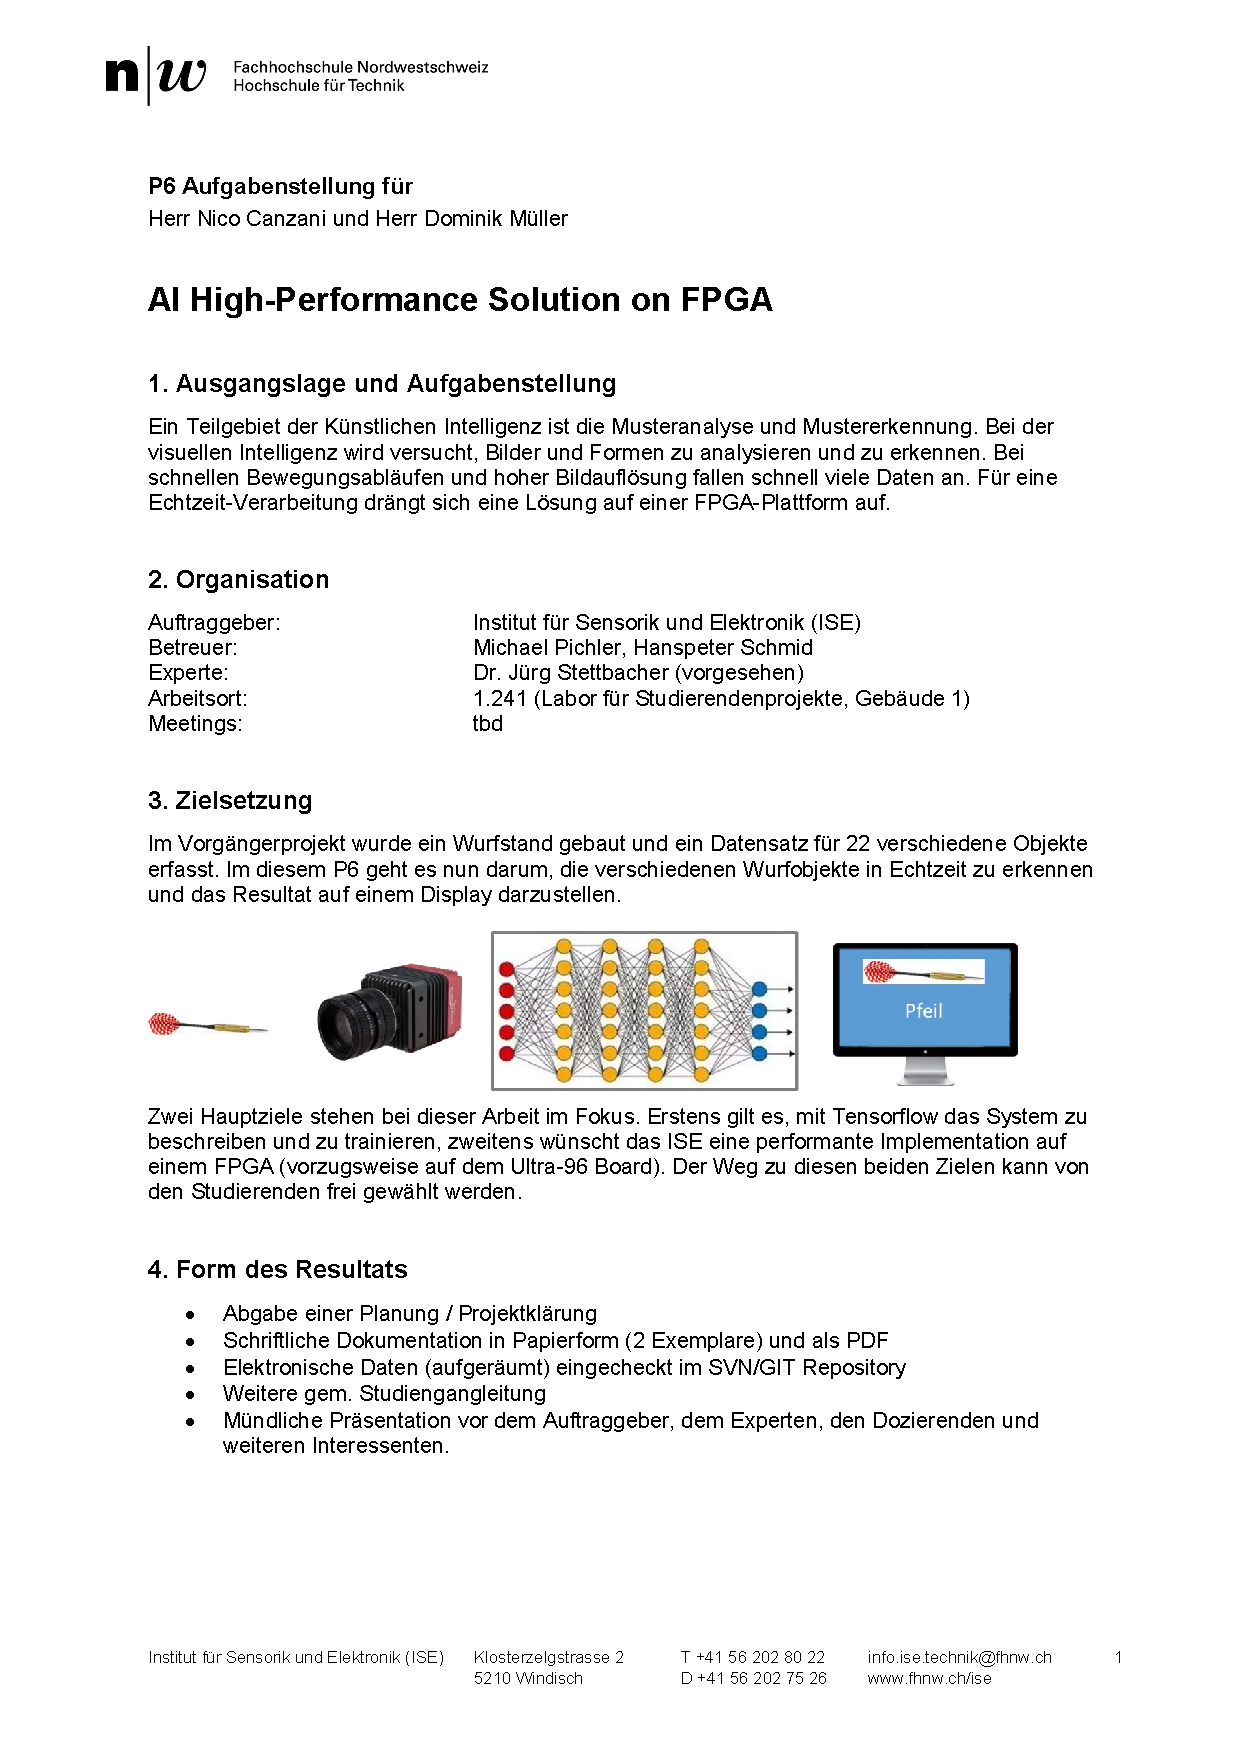
\includepdf[pages=-]{appendix/problem_statement.pdf}

  \chapter{Inference Application}
  \label{app:inference_application}
  \lstinputlisting[style=python]{appendix/aionfpga.py}
\end{appendix}


% Debug
%\newpage
%\listoftodos[\section{To-Do}]
%\clearpage

\end{document}
